%% LaTeX2e class for student theses
%% sections/evaluation.tex
%% 
%% Karlsruhe Institute of Technology
%% Institute for Program Structures and Data Organization
%% Chair for Software Design and Quality (SDQ)
%%
%% Dr.-Ing. Erik Burger
%% burger@kit.edu
%%
%% Version 1.3.6, 2022-09-28

\chapter{Evaluation}
\label{ch:Evaluation}

In the following chapter we will evaluate the experiments we conducted. We start off by explaining our evaluation metrics, both for Continual Active Learning
and when applying Continual Active Learning to Model Stealing. Afterwards we will present the results of our experiments and discuss the findings.

\section{Evaluation Metrics}
\label{sec:Evaluation:Metrics}
% Describe that we used agreement for model stealing (and on which dataset) and 
% validation accuracy for the model stealing experiments. and hyperparameters

\subsection{Metrics for Continual Active Learning}
\label{sec:Evaluation:Metrics:CAL}
When choosing a metric to evaluate Continual Active Learning, we need to remember the motivation of the approach. We proposed the Continual Active Learning approach
mainly to reduce the mainly to mitigate the overhead of pure Active Learning compared to the classic training loop. Therefore, it is desirable to incorporate a metric
which measures this goal. In our case, this is the overall execution time. However, execution time is not the only metric we want to use to evaluate the approach. Since 
the second goal of the Continual Learning approach is to improve model performance, we will also evaluate the experiments based on this. What a makes a machine learning 
model performant has been discussed vividly in the literature. In our case, we will use the validation accuracy as a metric to evaluate the performance of the model. It is
important to consider \textit{both} runtime and validation accuracy when evaluating the experiments. A model with low runtime and low validation accuracy is not desirable,
but neither is a model with high runtime and high validation accuracy. Since we are trying to improve Active Learning by introducing Continual Learning into the pool-based 
Active Learning process, we aim to outperform the classic pool-based Active Learning approach. More precisely, we want to reduce the runtime and increase the validation
accuracy. The success of our Continual Active Learning approach will be evaluated against the classic pool-based Active Learning approach based on the runtime improvement
and the accuracy improvement. 


\subsection{Metrics for Continual Active Learning for Model Stealing}
\label{sec:Evaluation:Metrics:CALMS}
As presented in section \ref{sec:ModelStealing:Attacks}, Model Stealing Attacks can be performed for a variety of reasons. As we build our framework on ActiveThief, we also
adopt the metrics used in the original paper. The ActiveThief framework aims purely at stealing the functionality of the model, i.e. approximation the model's relationship
between input and output best, and so does ours. Therefore, we will use the same evaluation metric, which in our case is the agreement between substitute and target model,
computed on the validation split of the target model dataset. The baseline which we compare our results against is the ActiveThief framework. We will therefore measure the 
success of using Continual Active Learning for Model Stealing by comparing the model agreement of our approach to the model agreement of the ActiveThief framework.

\section{Results}
\label{sec:Evaluation:Results}
In this section we will present the results of our experiments. As mentioned before, our experiments are split into two parts. The first part is the evaluation of our novel
Continual Active Learning Approach and the second part is evaluating the performance our the Continual Active Learning approach when applied to Model Stealing. In each of these
respective subsections we will first describe the experiments schedule for each part and then present the results of the experiments.

\subsection{Results for Continual Active Learning}
\label{sec:Evaluation:Results:CAL}
In this subsection we will first present

\begin{figure} [ht]
    \centering
    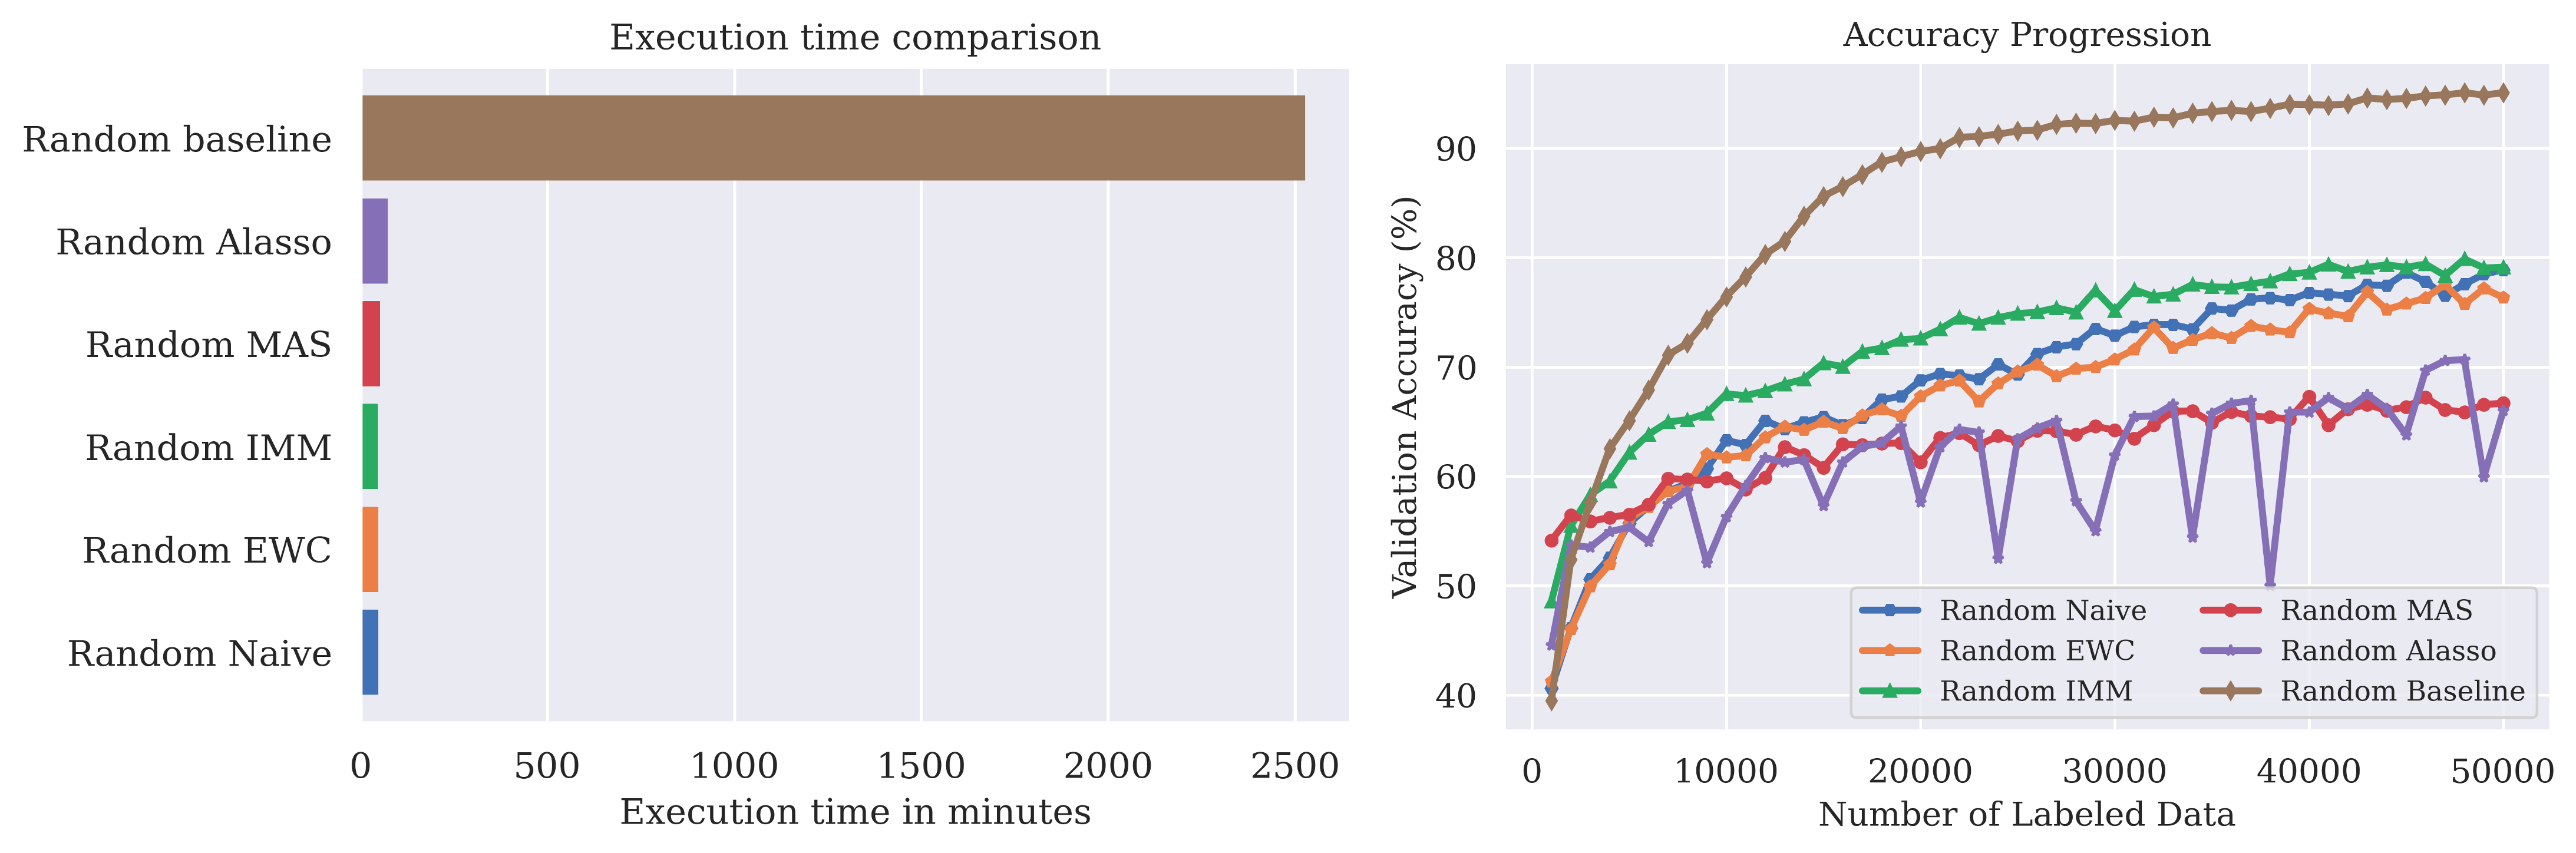
\includegraphics[width=\linewidth]{images/results_CAL/Random_CAL_1000b.png}
    \caption[Continual Active Learning Random 1000 batch size]{A}
    \label{fig:Evaluation:Results:CAL:Random1000}
\end{figure}

\begin{figure} [ht]
    \centering
    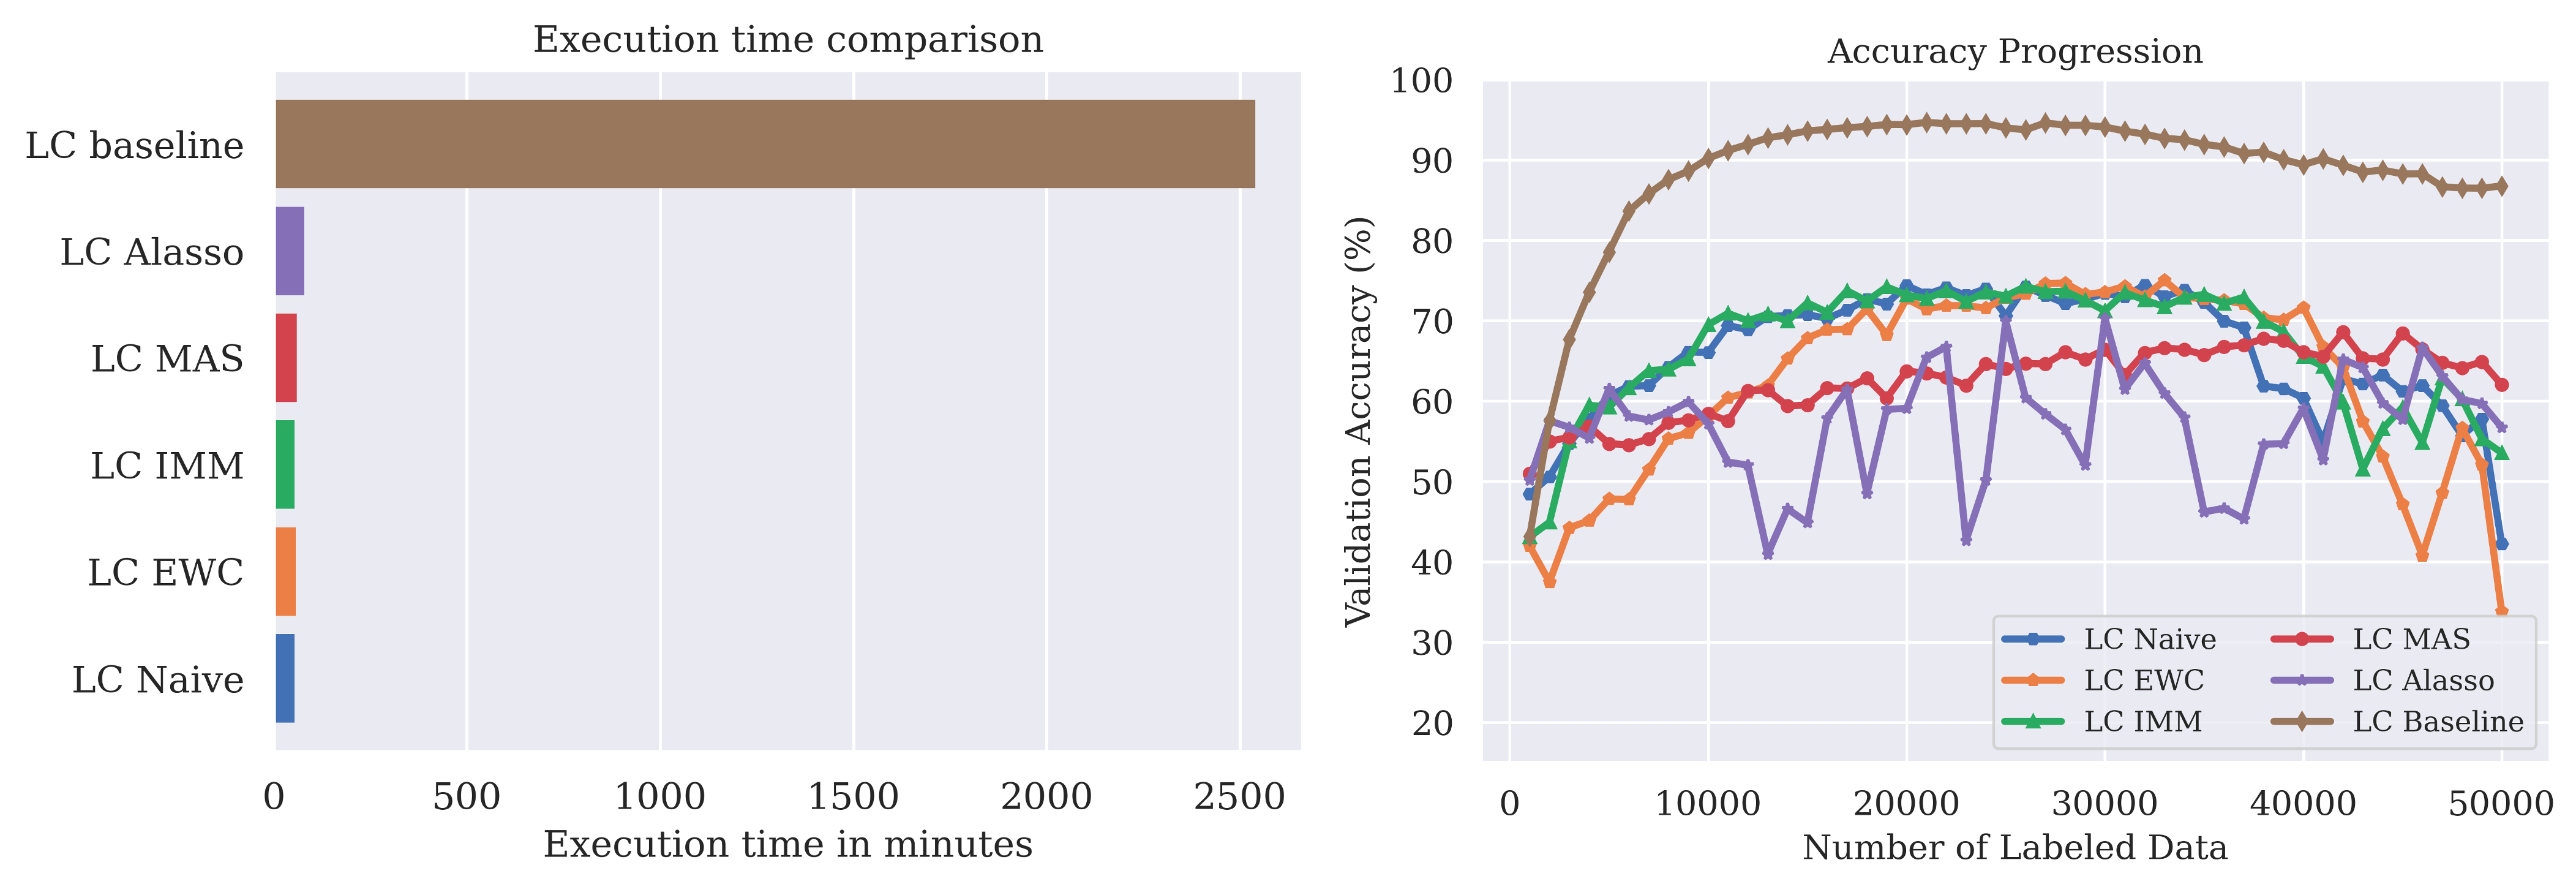
\includegraphics[width=\linewidth]{images/results_CAL/LC_CAL_1000b.png}
    \caption[Continual Active Learning Random 1000 batch size]{B}
    \label{fig:Evaluation:Results:CAL:LC1000}
\end{figure}

\begin{figure} [ht]
    \centering
    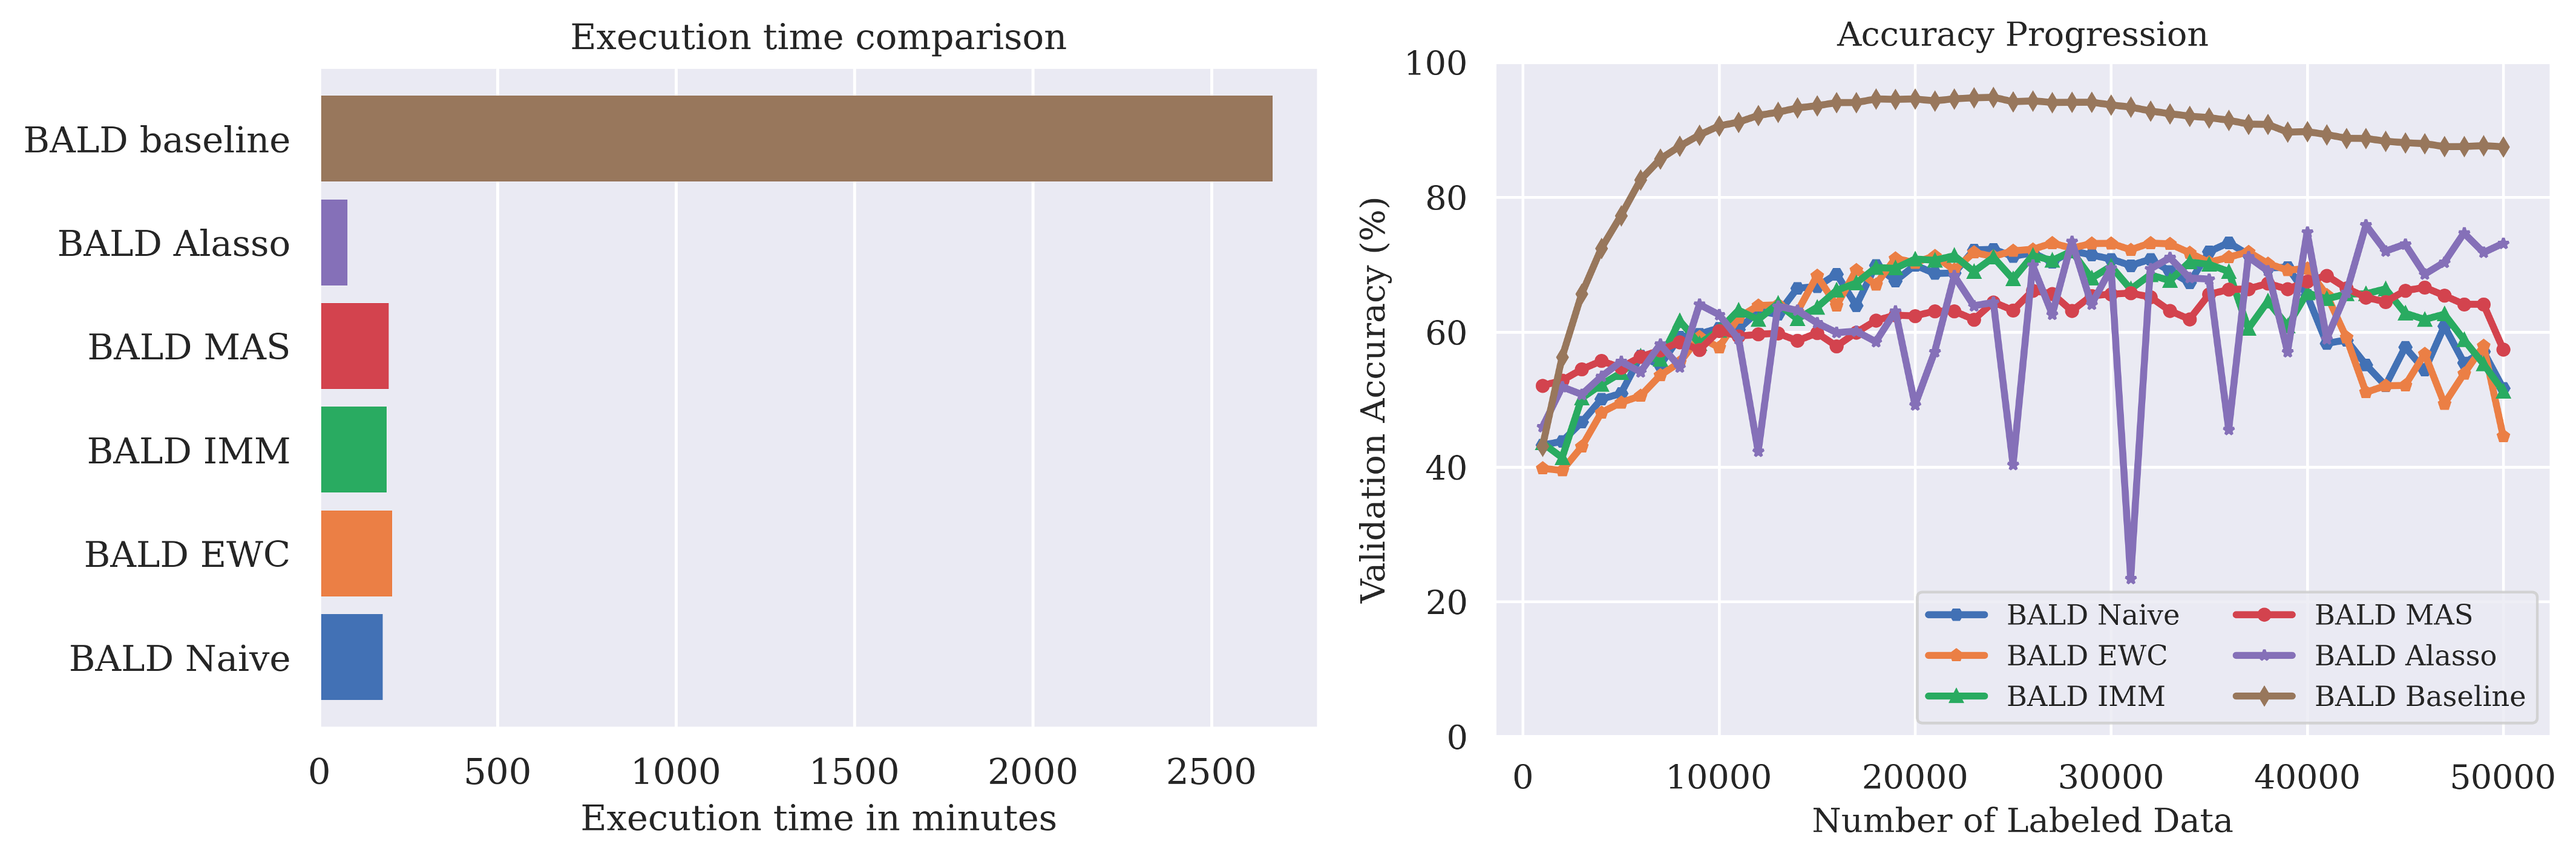
\includegraphics[width=\linewidth]{images/results_CAL/Bald_CAL_1000b.png}
    \caption[Continual Active Learning BALD 1000 batch size]{C}
    \label{fig:Evaluation:Results:CAL:BALD1000}
\end{figure}

\begin{figure} [ht]
    \centering
    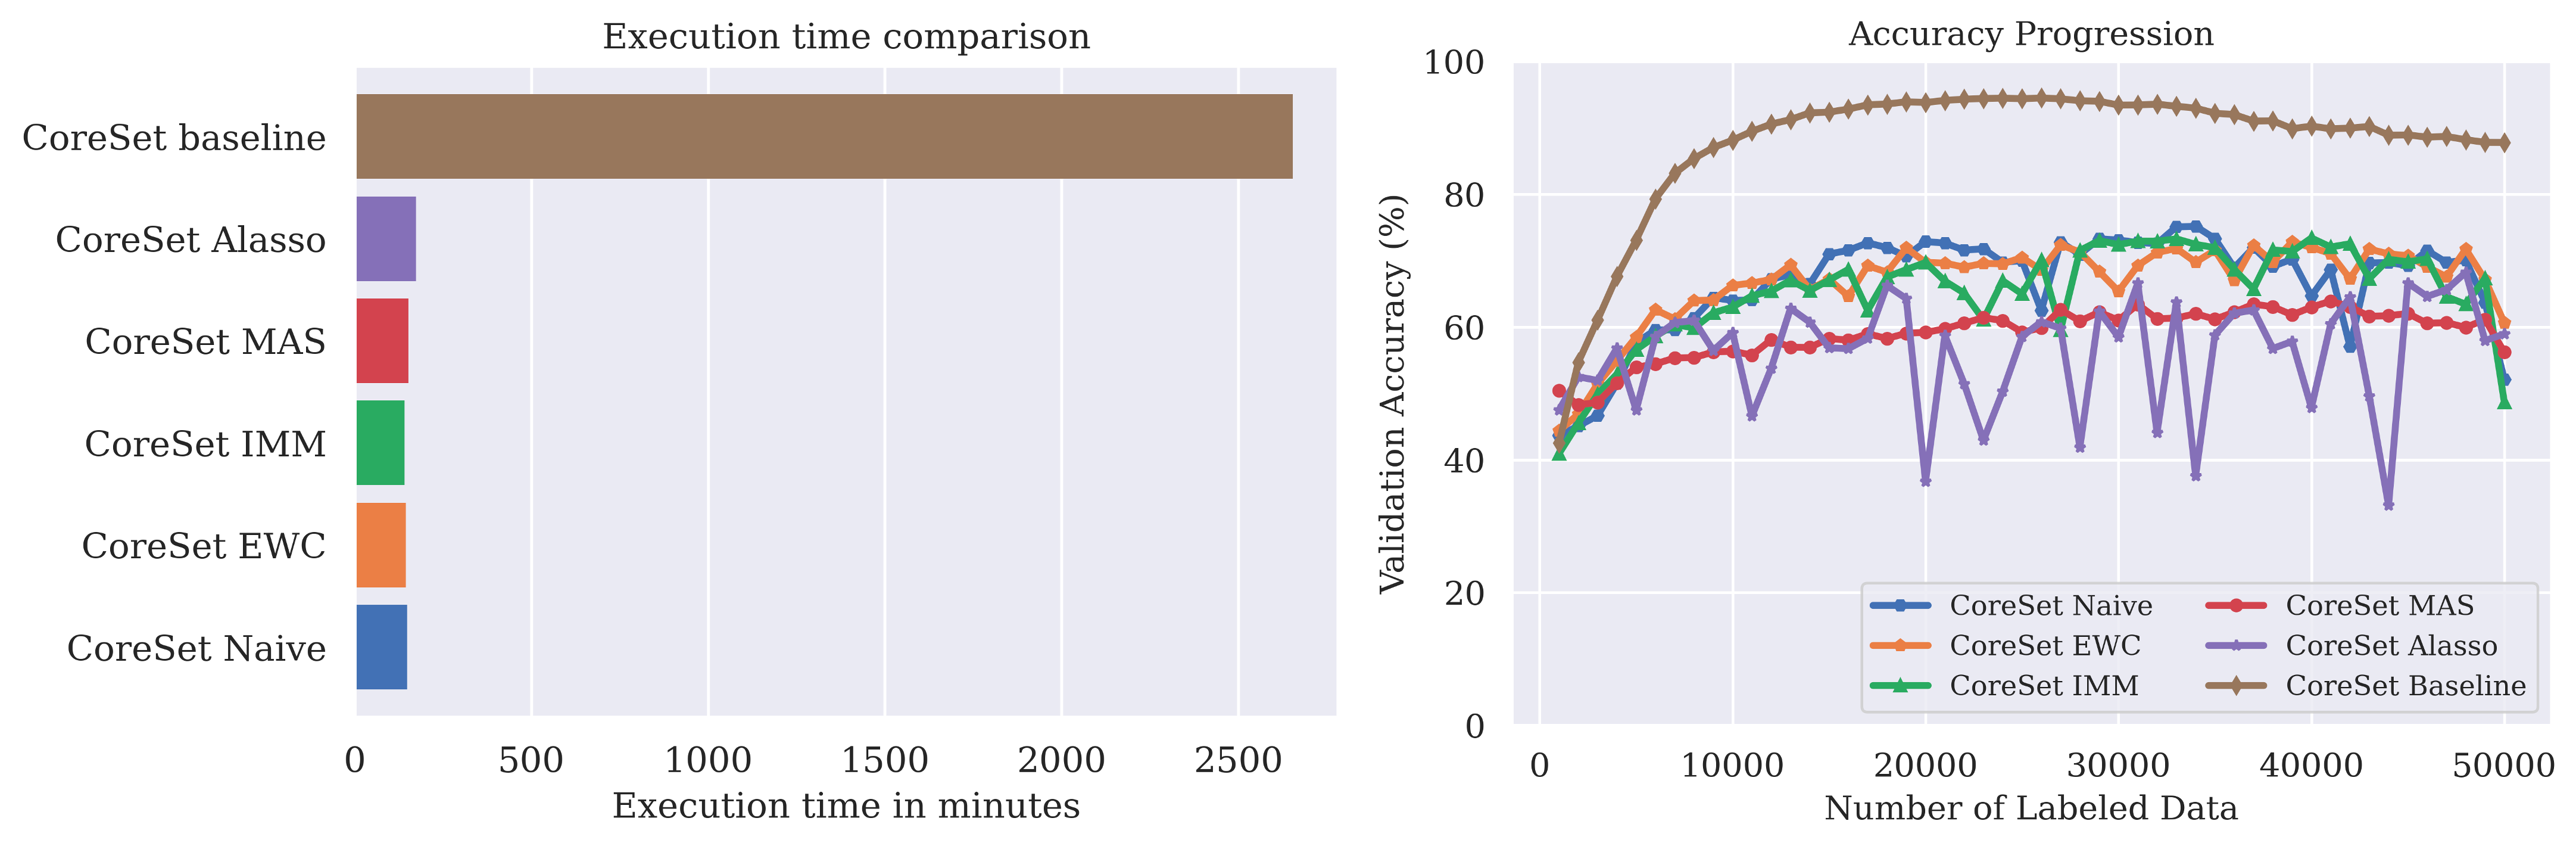
\includegraphics[width=\linewidth]{images/results_CAL/CoreSet_CAL_1000b.png}
    \caption[Continual Active Learning CoreSet 1000 batch size]{D}
    \label{fig:Evaluation:Results:CAL:CoreSet1000}
\end{figure}

\begin{figure} [ht]
    \centering
    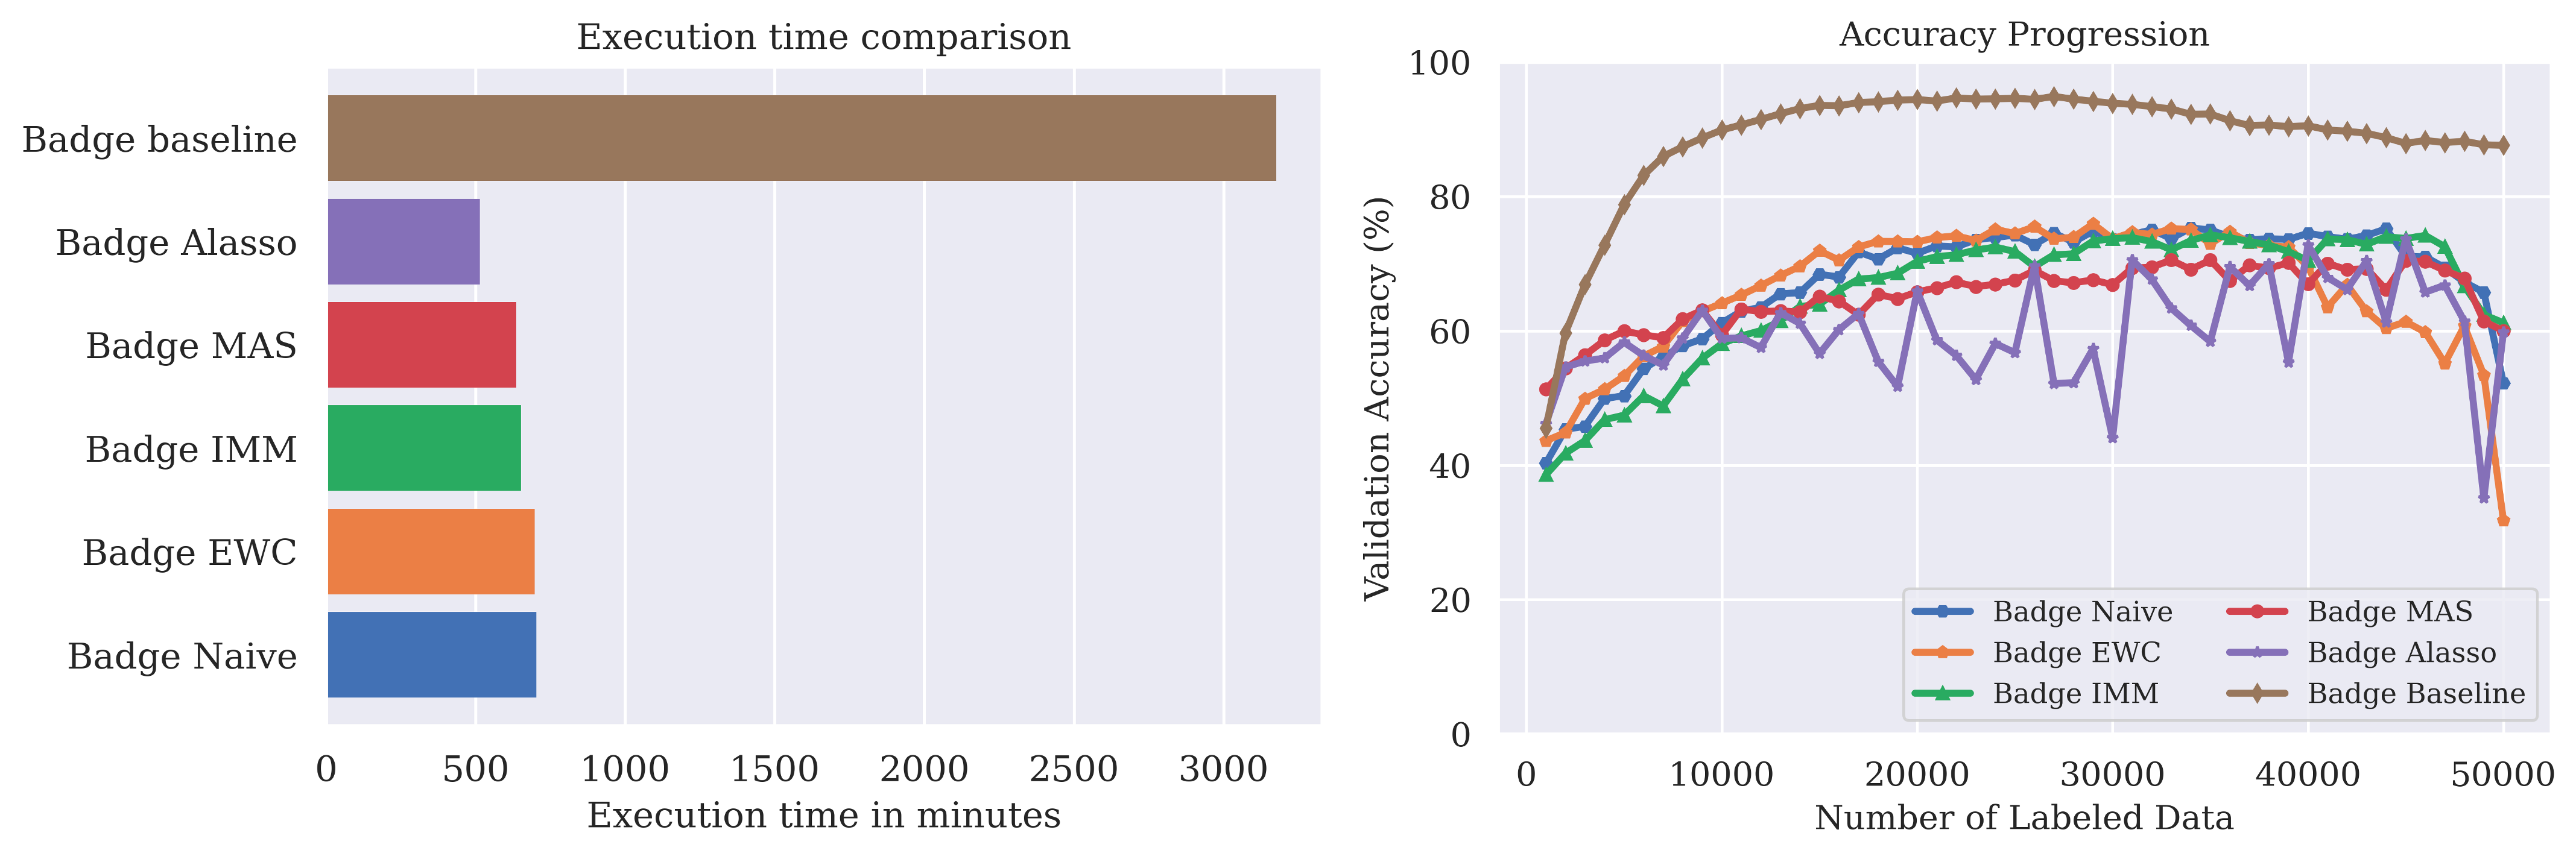
\includegraphics[width=\linewidth]{images/results_CAL/Badge_CAL_1000b.png}
    \caption[Continual Active Learning Badge 1000 batch size]{E}
    \label{fig:Evaluation:Results:CAL:Badge1000}
\end{figure}




\begin{figure} [ht]
    \centering
    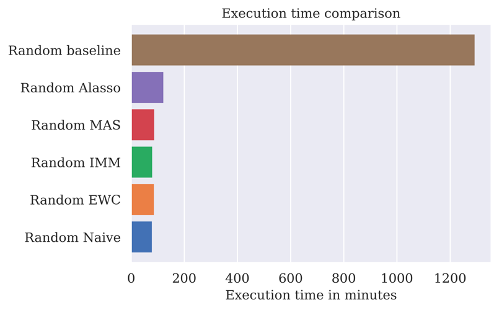
\includegraphics[width=\linewidth]{images/results_CAL/Random_CAL_2000b.png}
    \caption[Continual Active Learning Random 2000 batch size]{A}
    \label{fig:Evaluation:Results:CAL:Random2000}
\end{figure}

\begin{figure} [ht]
    \centering
    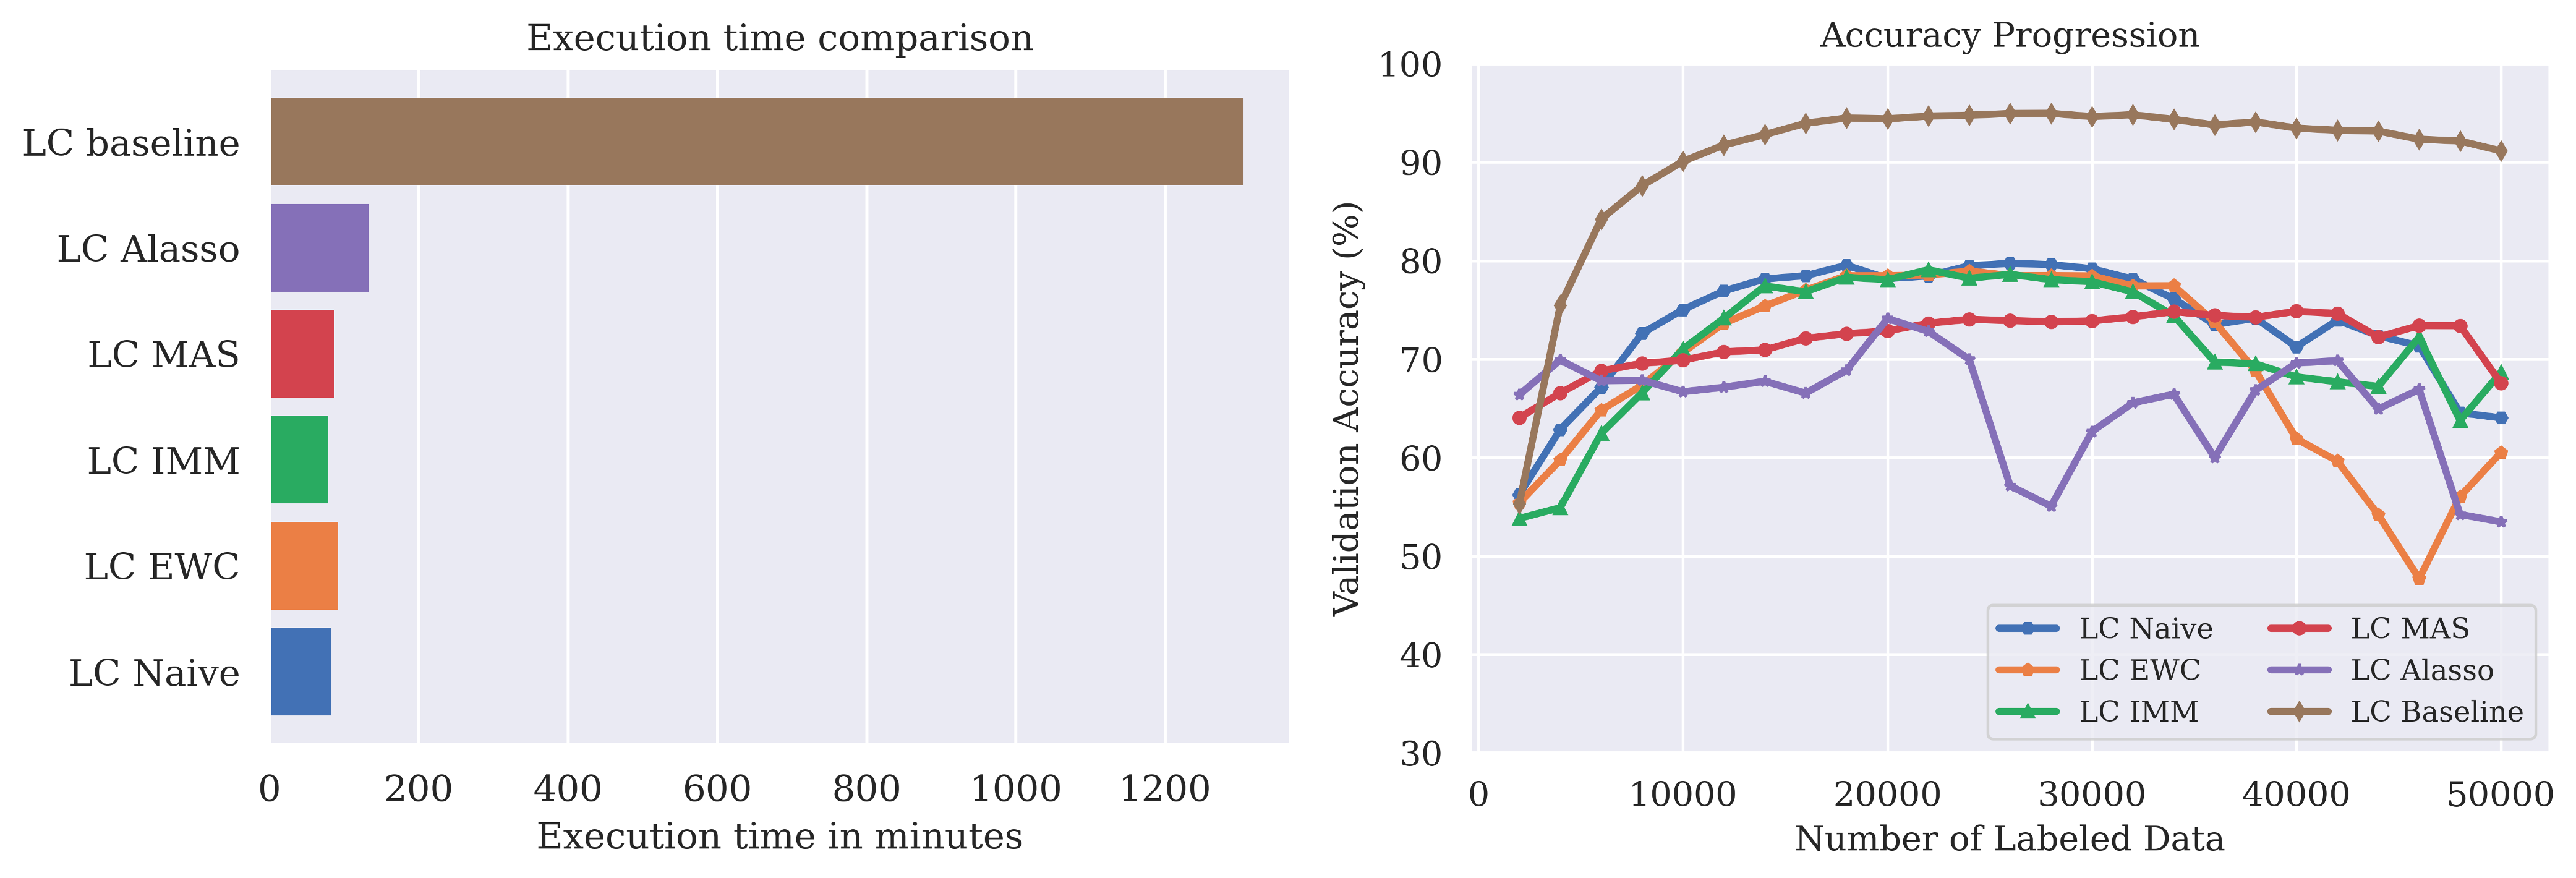
\includegraphics[width=\linewidth]{images/results_CAL/LC_CAL_2000b.png}
    \caption[Continual Active Learning Random 2000 batch size]{B}
    \label{fig:Evaluation:Results:CAL:LC2000}
\end{figure}

\begin{figure} [ht]
    \centering
    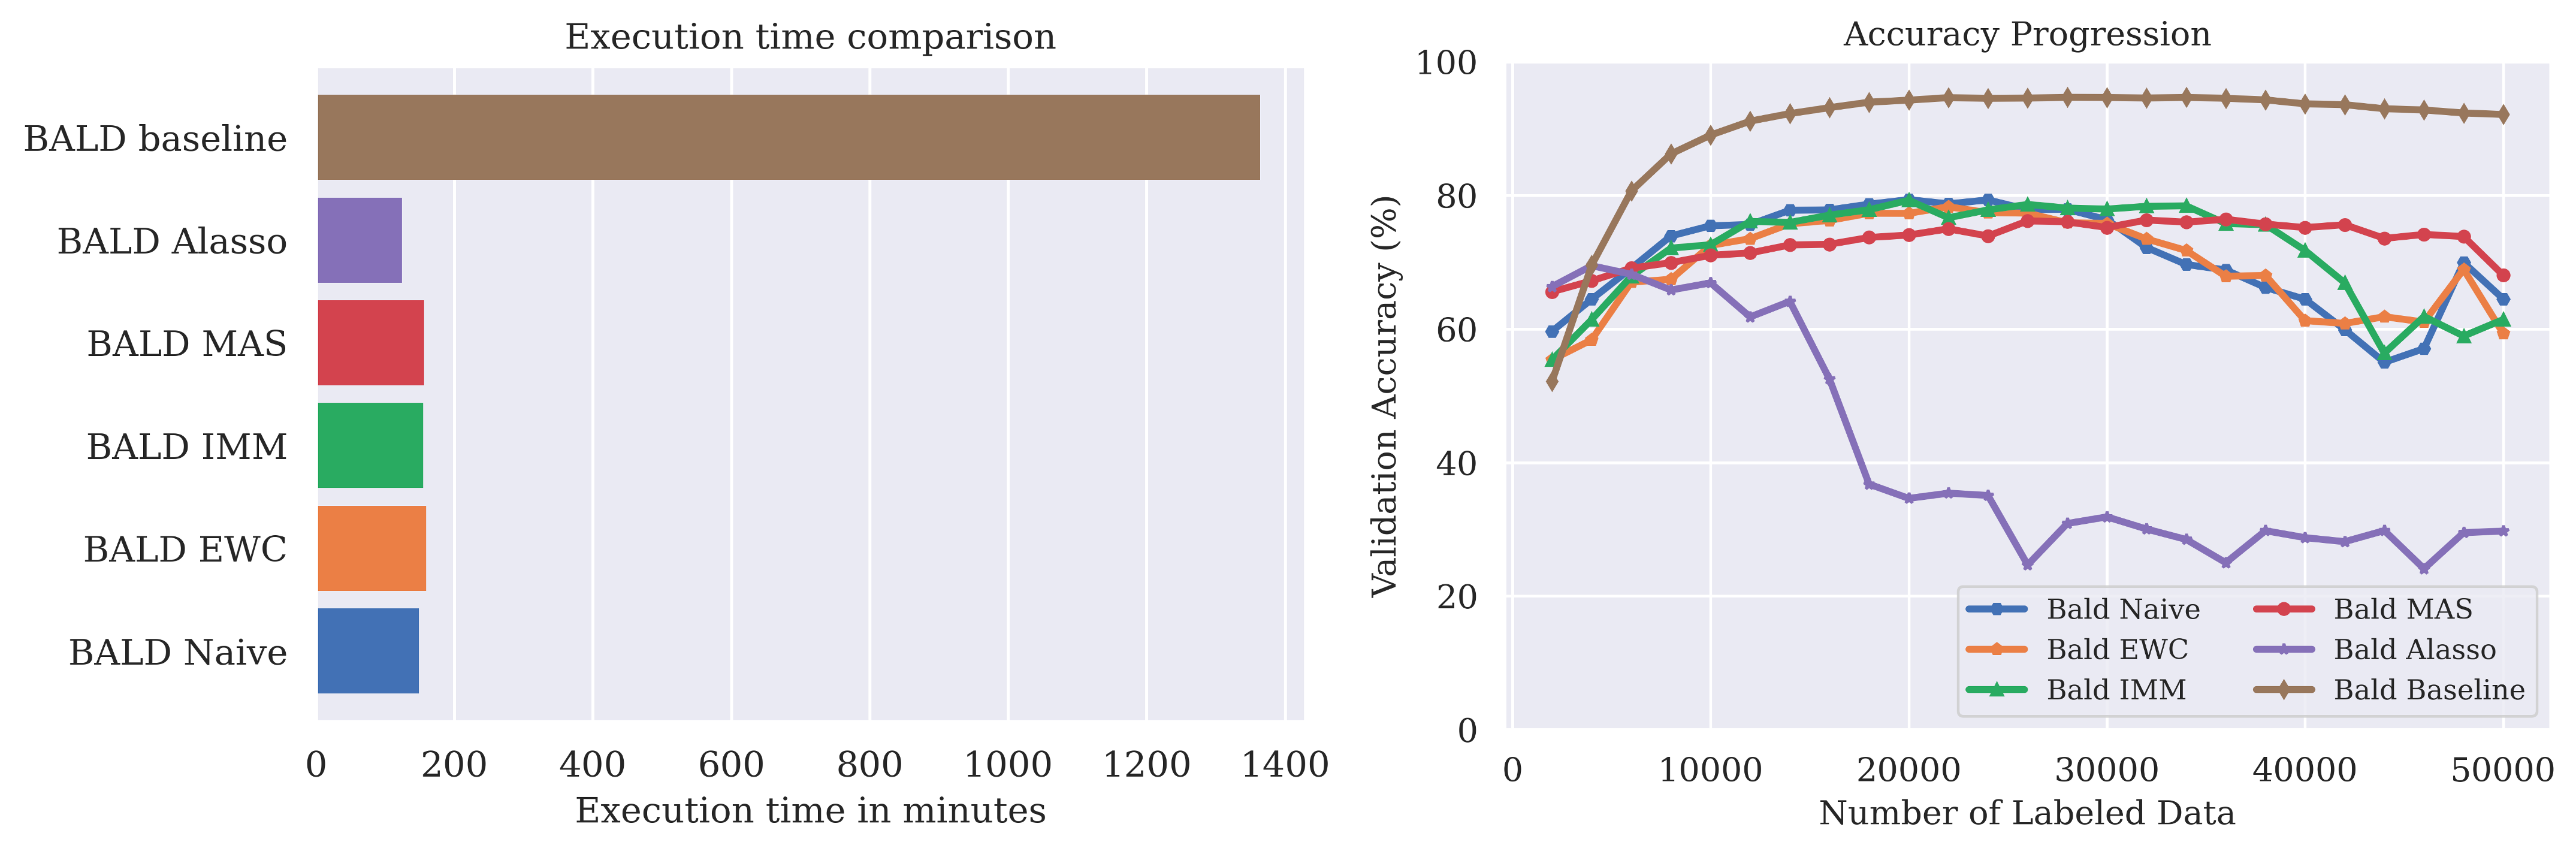
\includegraphics[width=\linewidth]{images/results_CAL/Bald_CAL_2000b.png}
    \caption[Continual Active Learning BALD 2000 batch size]{C}
    \label{fig:Evaluation:Results:CAL:BALD2000}
\end{figure}

\begin{figure} [ht]
    \centering
    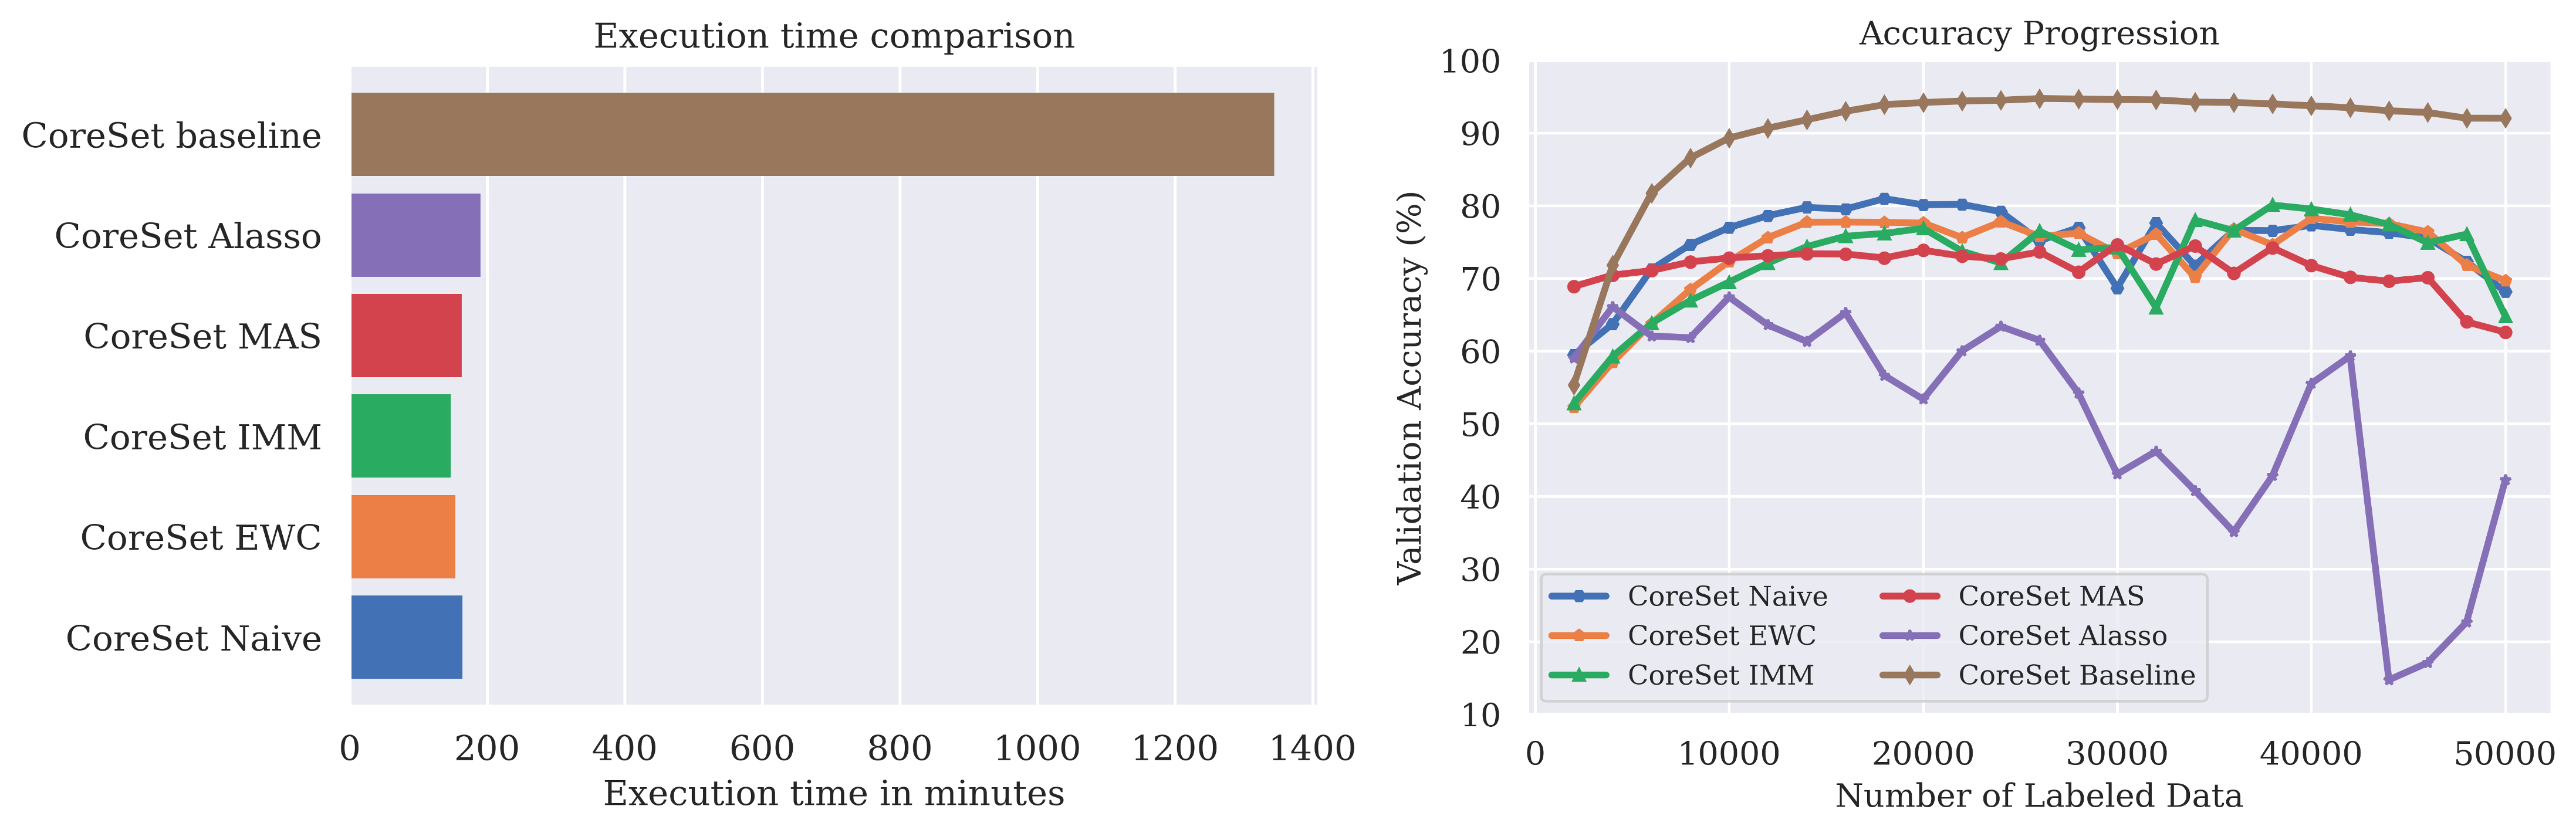
\includegraphics[width=\linewidth]{images/results_CAL/CoreSet_CAL_2000b.png}
    \caption[Continual Active Learning CoreSet 2000 batch size]{D}
    \label{fig:Evaluation:Results:CAL:CoreSet2000}
\end{figure}

\begin{figure} [ht]
    \centering
    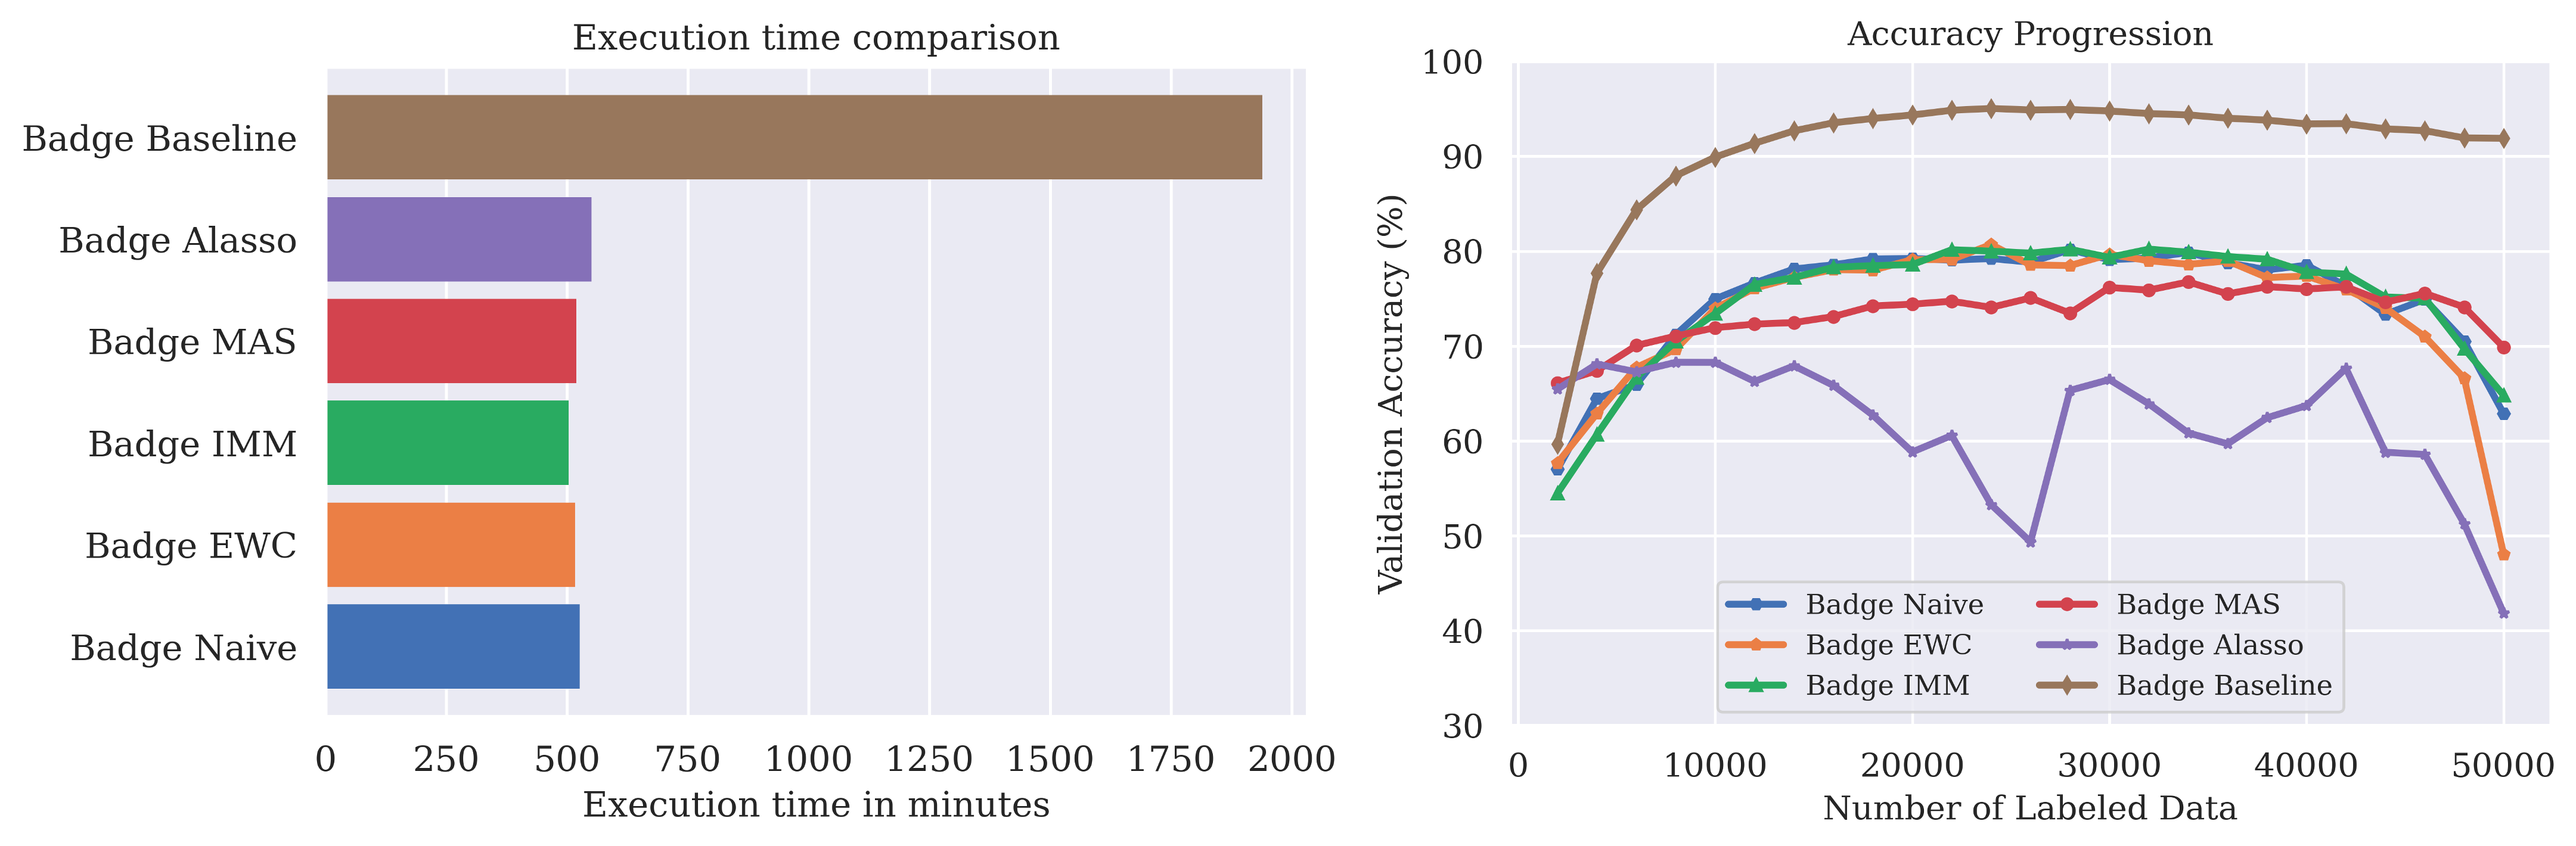
\includegraphics[width=\linewidth]{images/results_CAL/Badge_CAL_2000b.png}
    \caption[Continual Active Learning Badge 2000 batch size]{E}
    \label{fig:Evaluation:Results:CAL:Badge2000}
\end{figure}





\begin{figure} [ht]
    \centering
    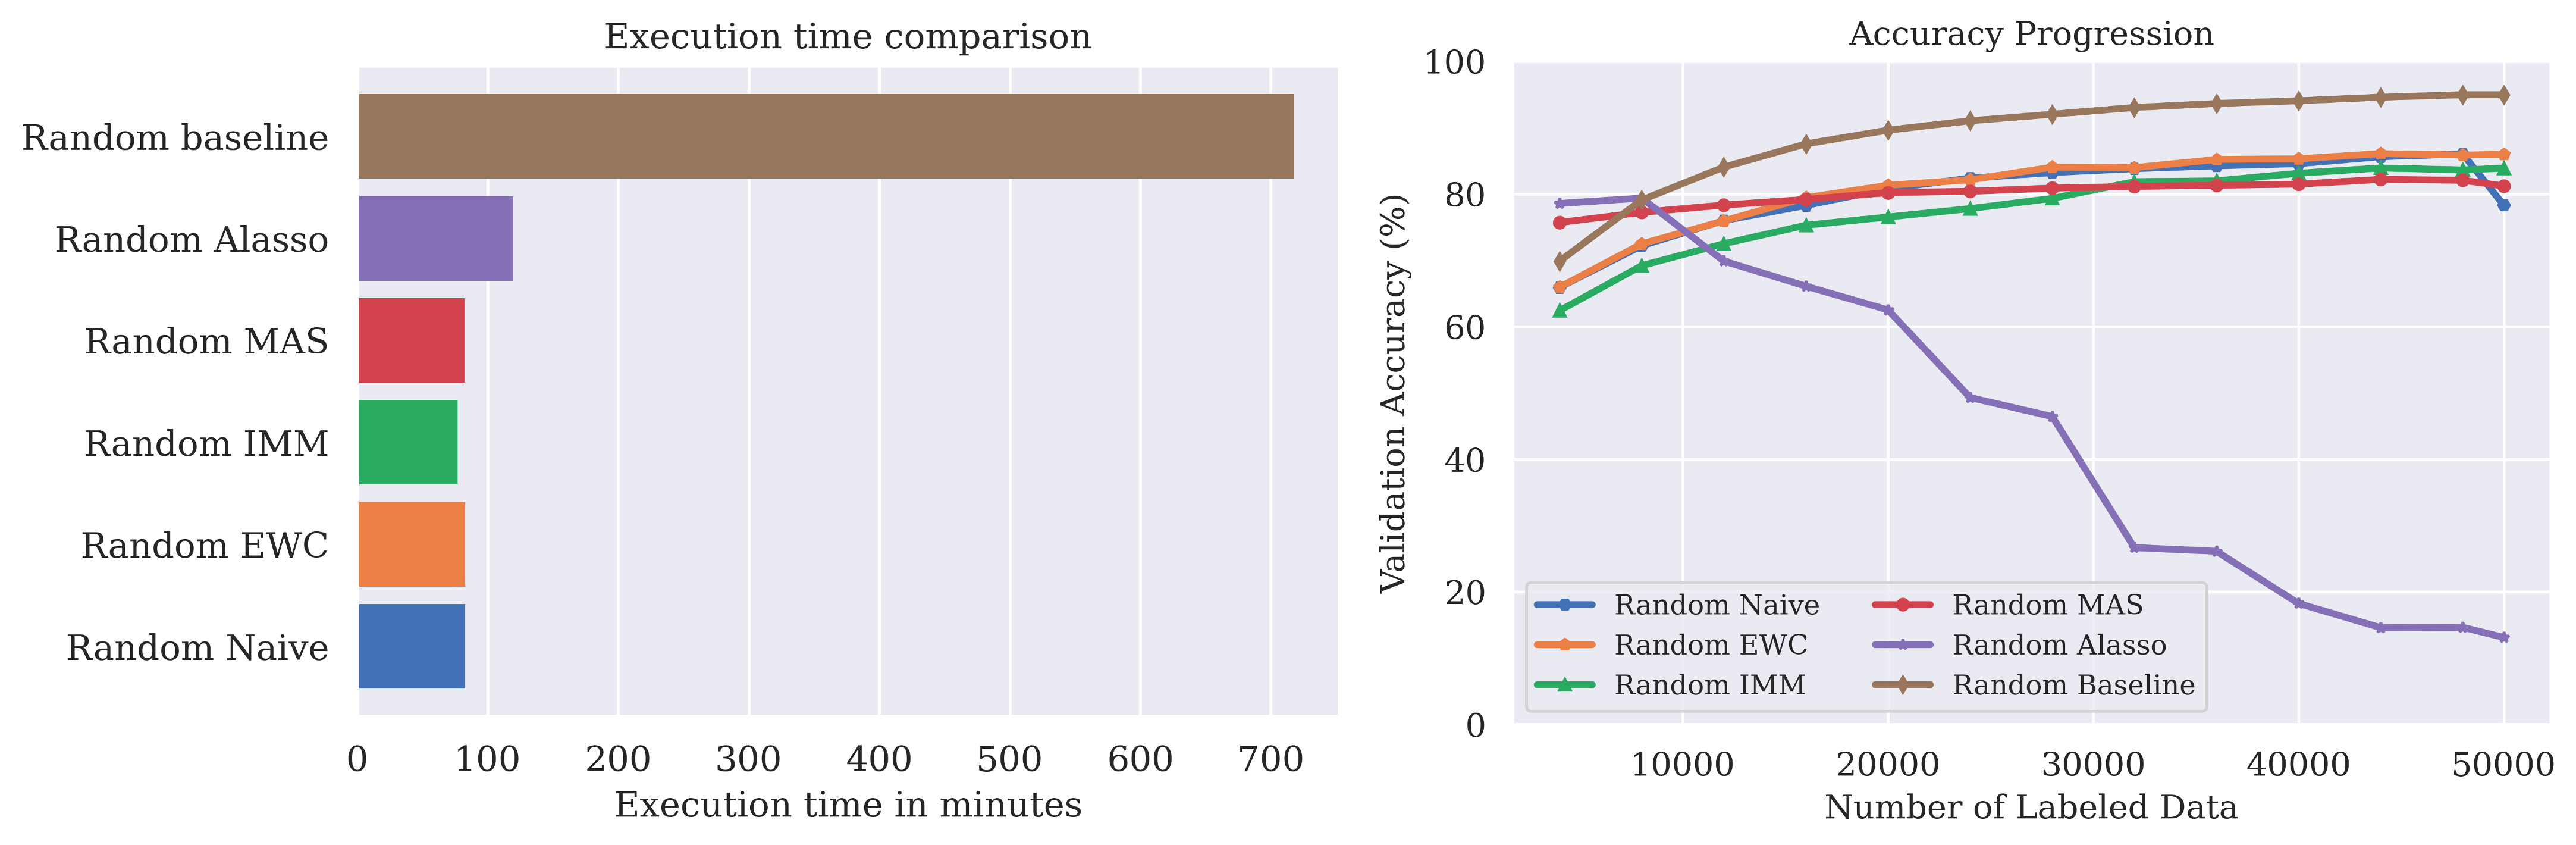
\includegraphics[width=\linewidth]{images/results_CAL/Random_CAL_4000b.png}
    \caption[Continual Active Learning Random 4000 batch size]{A}
    \label{fig:Evaluation:Results:CAL:Random4000}
\end{figure}

\begin{figure} [ht]
    \centering
    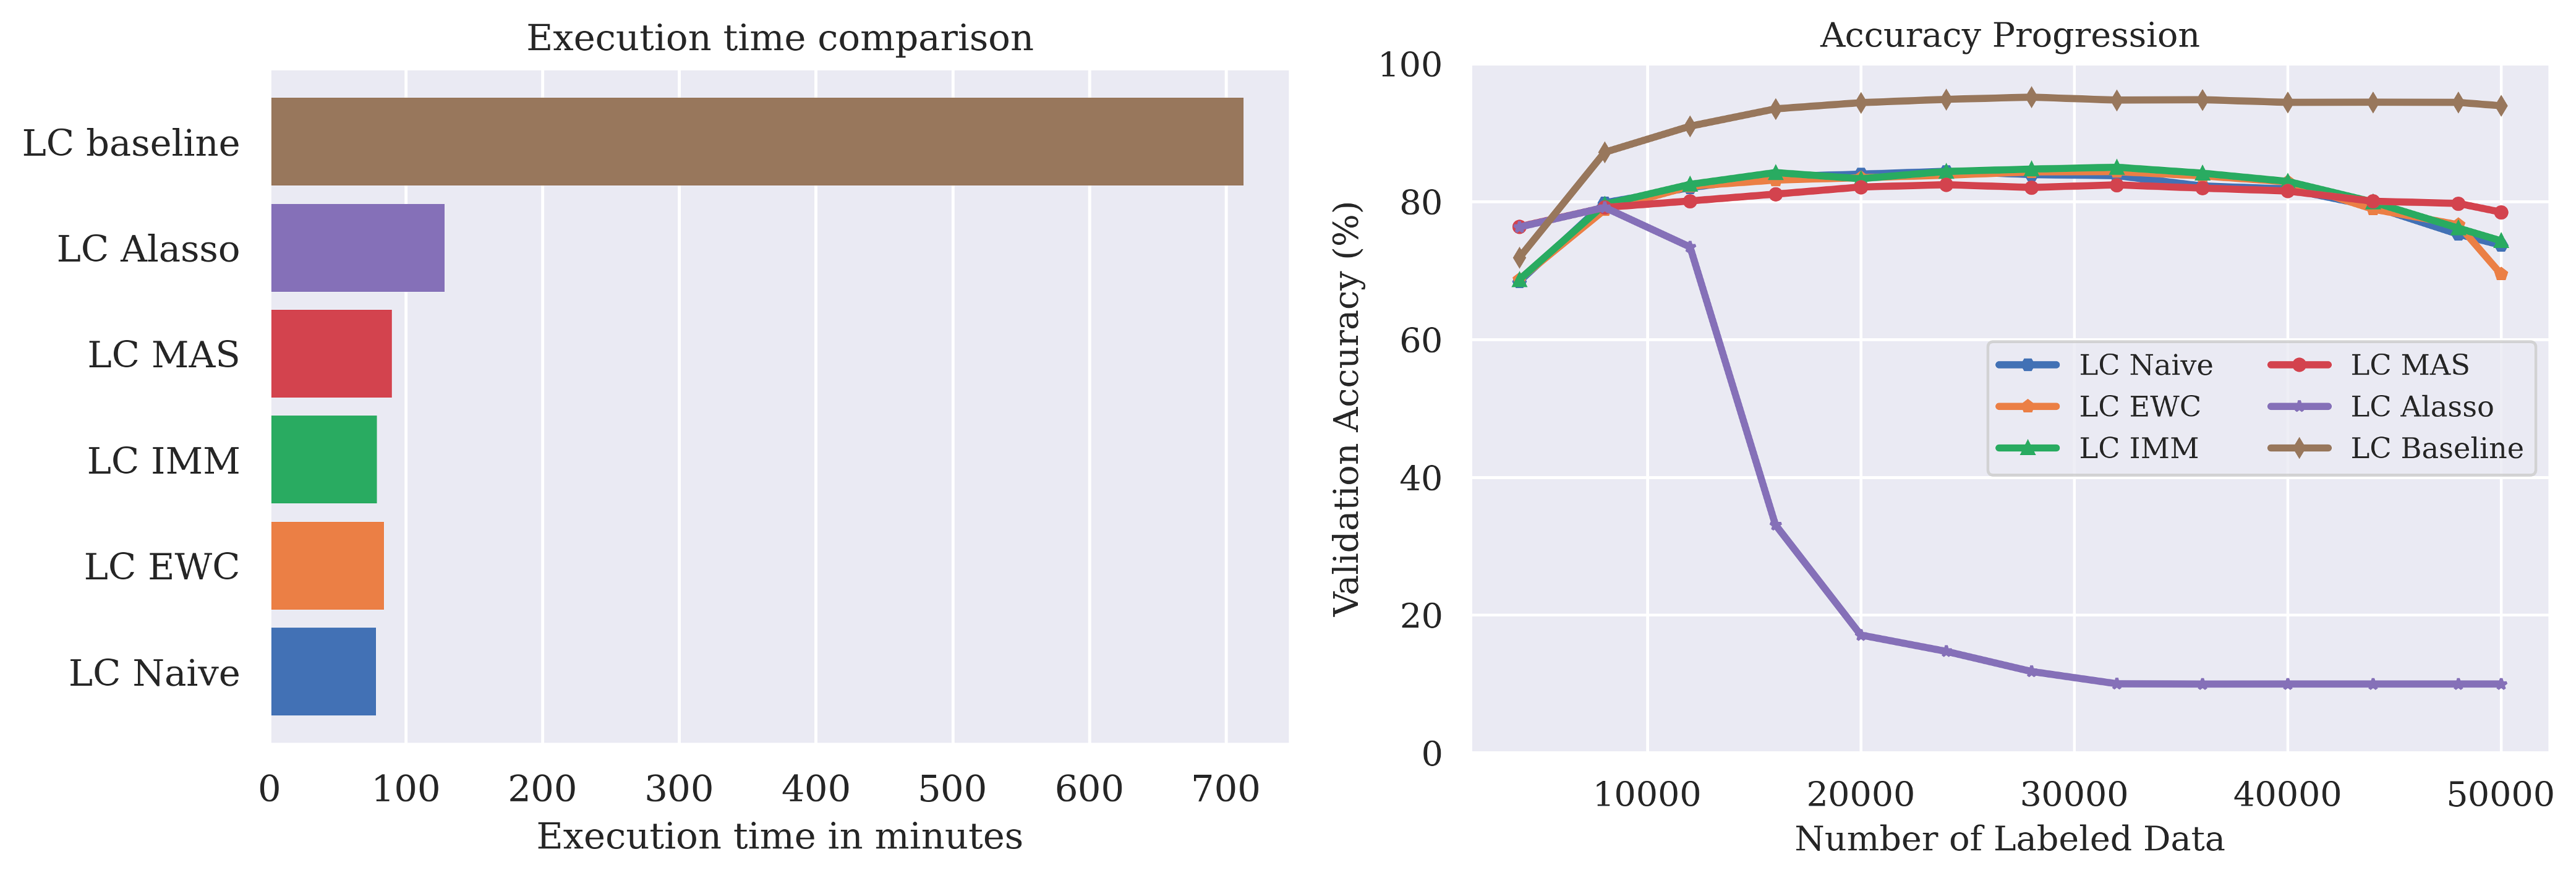
\includegraphics[width=\linewidth]{images/results_CAL/LC_CAL_4000b.png}
    \caption[Continual Active Learning Random 4000 batch size]{B}
    \label{fig:Evaluation:Results:CAL:LC4000}
\end{figure}

\begin{figure} [ht]
    \centering
    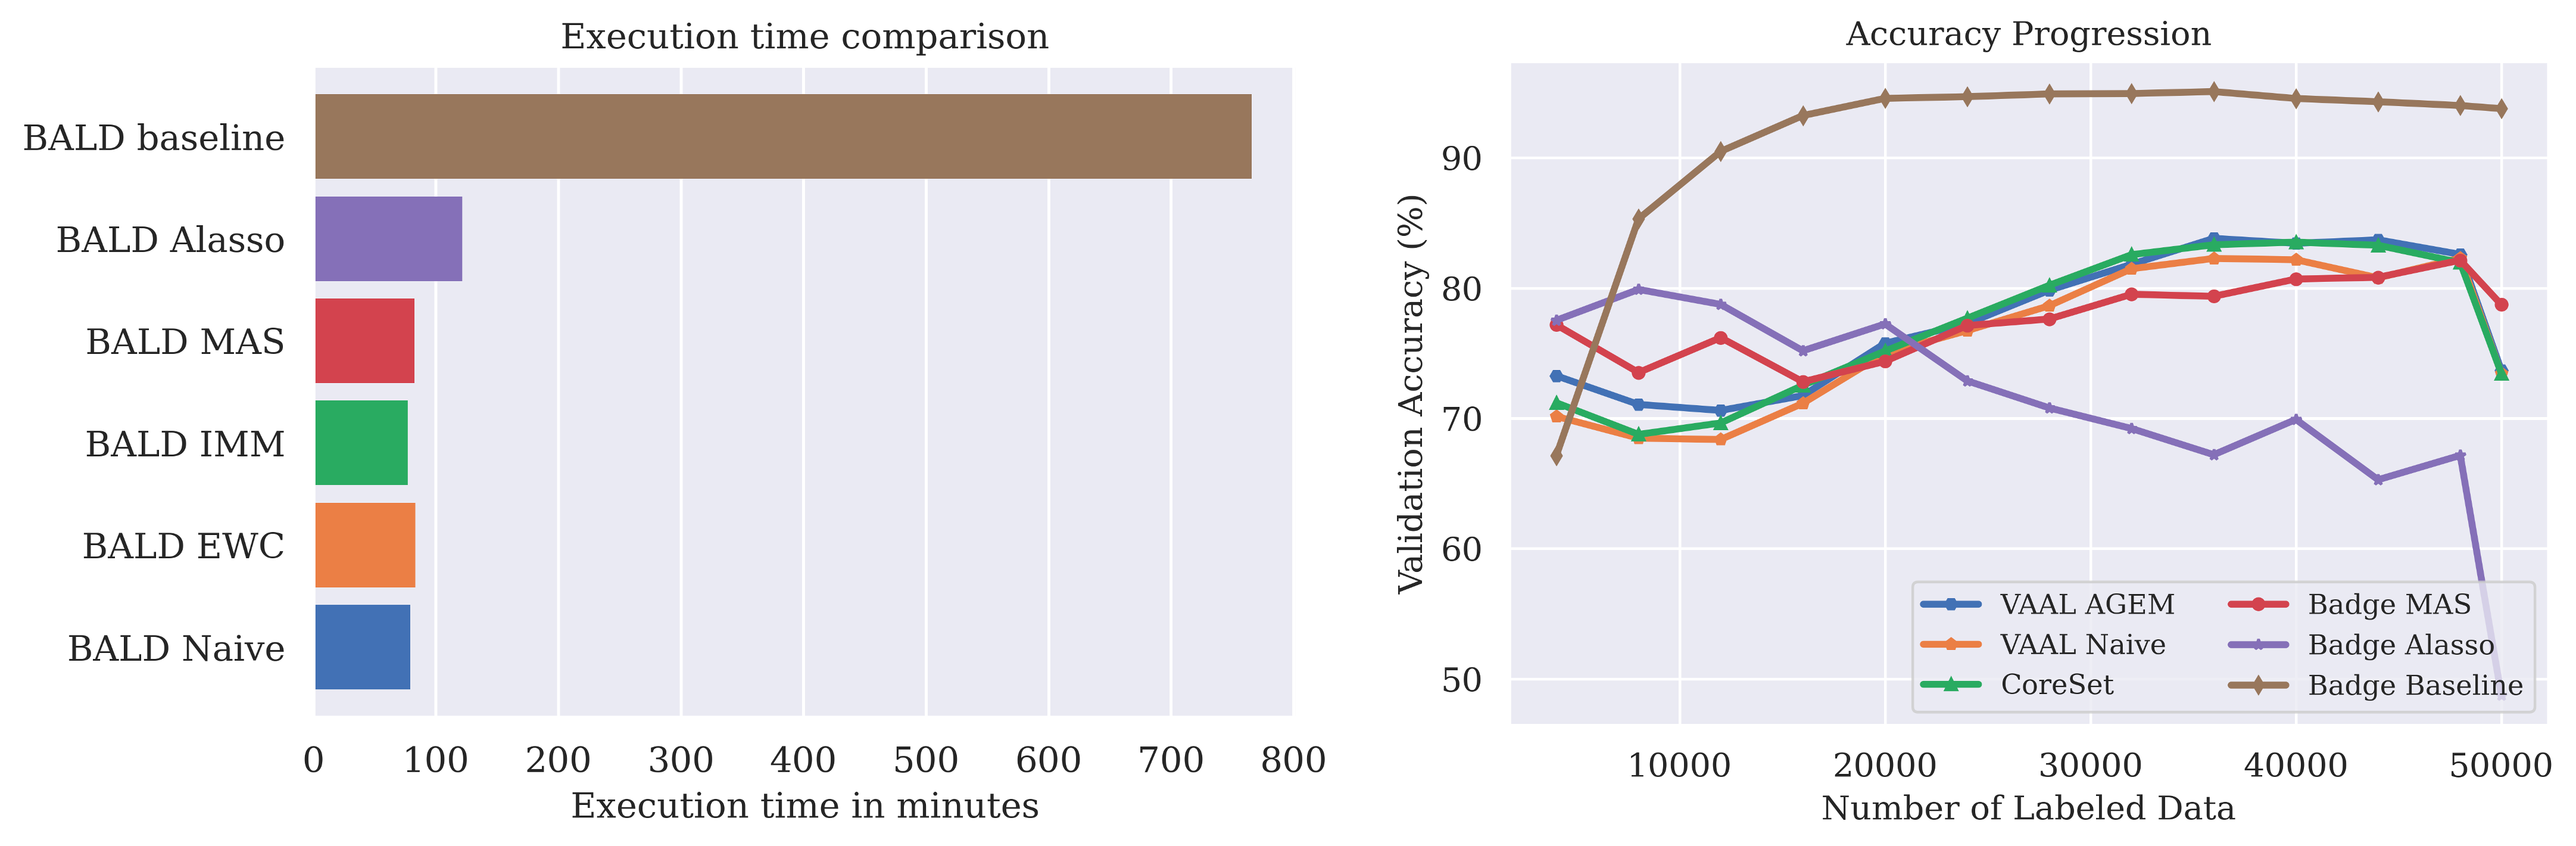
\includegraphics[width=\linewidth]{images/results_CAL/Bald_CAL_4000b.png}
    \caption[Continual Active Learning BALD 4000 batch size]{C}
    \label{fig:Evaluation:Results:CAL:BALD4000}
\end{figure}

\begin{figure} [ht]
    \centering
    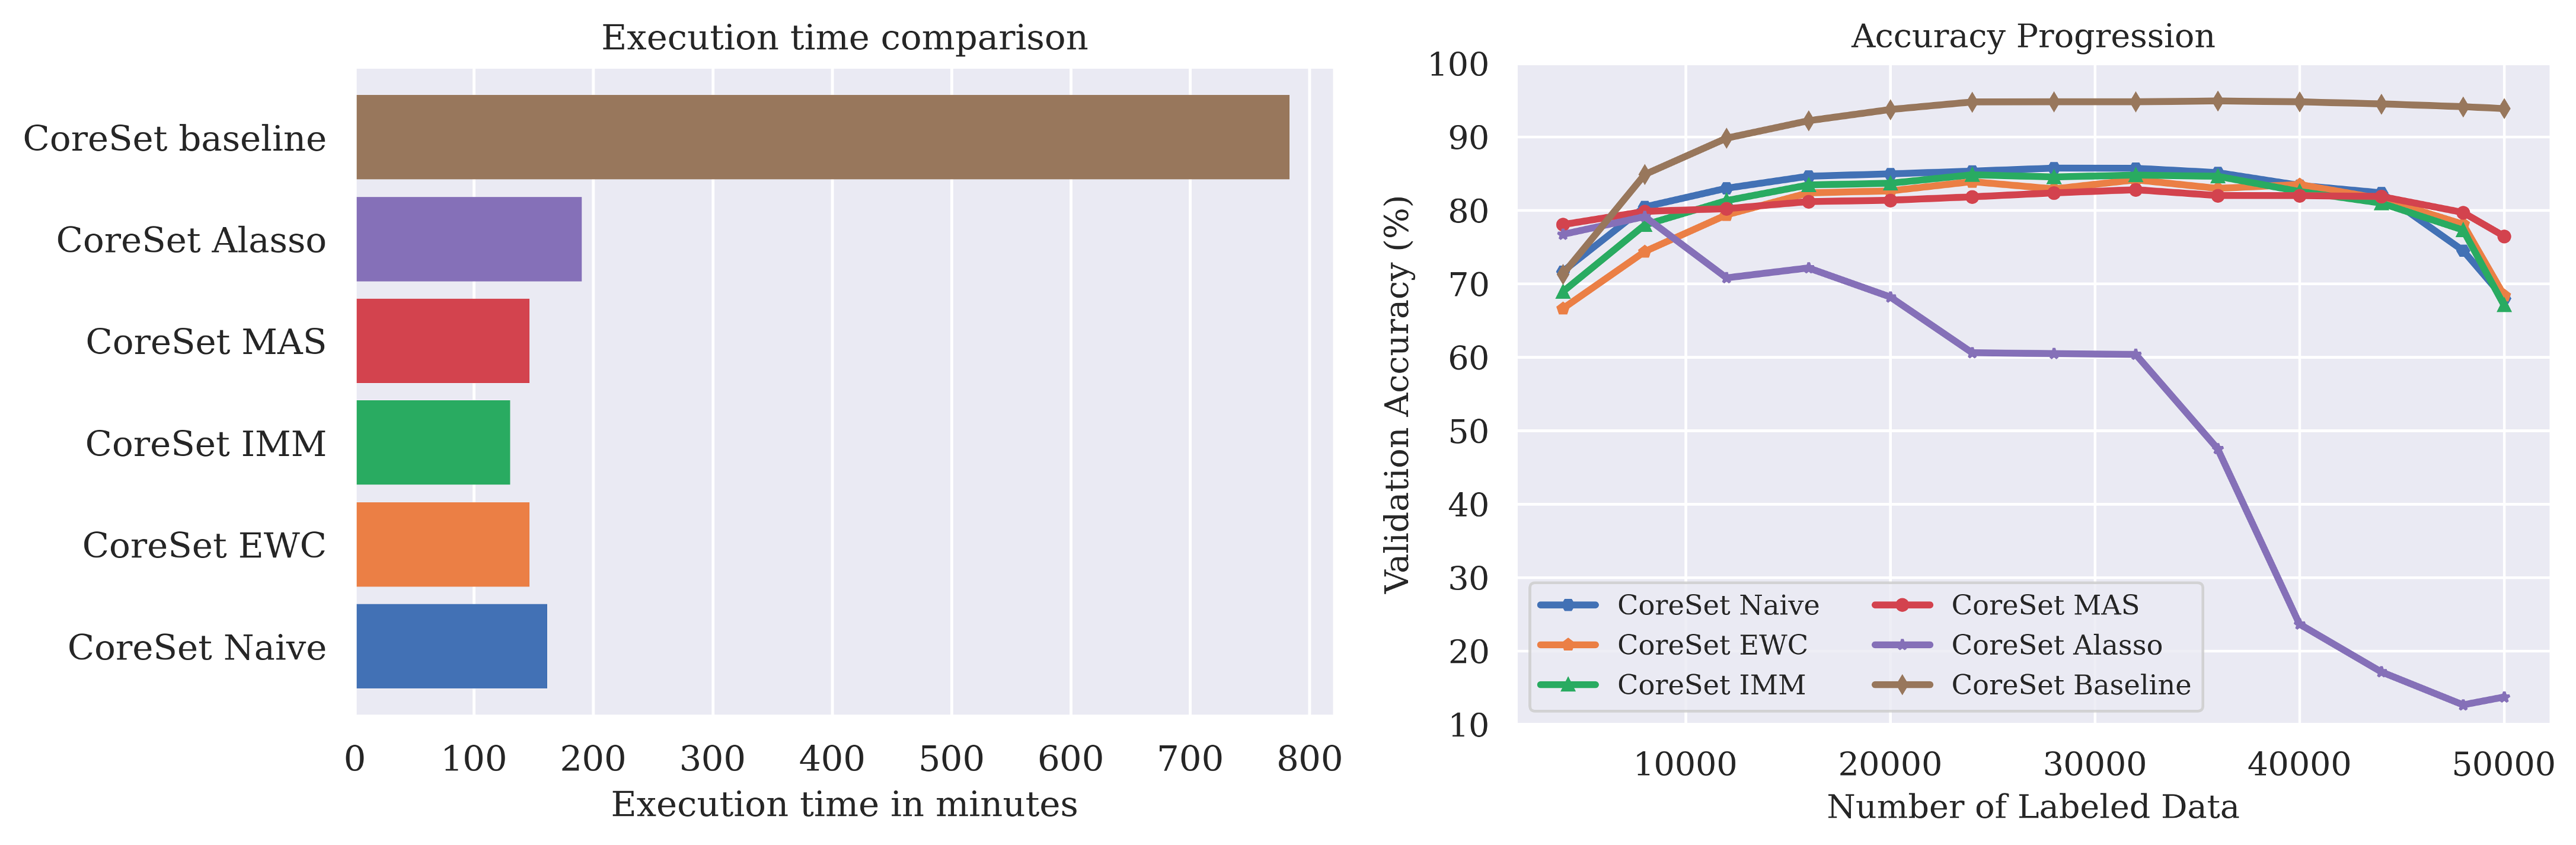
\includegraphics[width=\linewidth]{images/results_CAL/CoreSet_CAL_4000b.png}
    \caption[Continual Active Learning CoreSet 4000 batch size]{D}
    \label{fig:Evaluation:Results:CAL:CoreSet4000}
\end{figure}

\begin{figure} [ht]
    \centering
    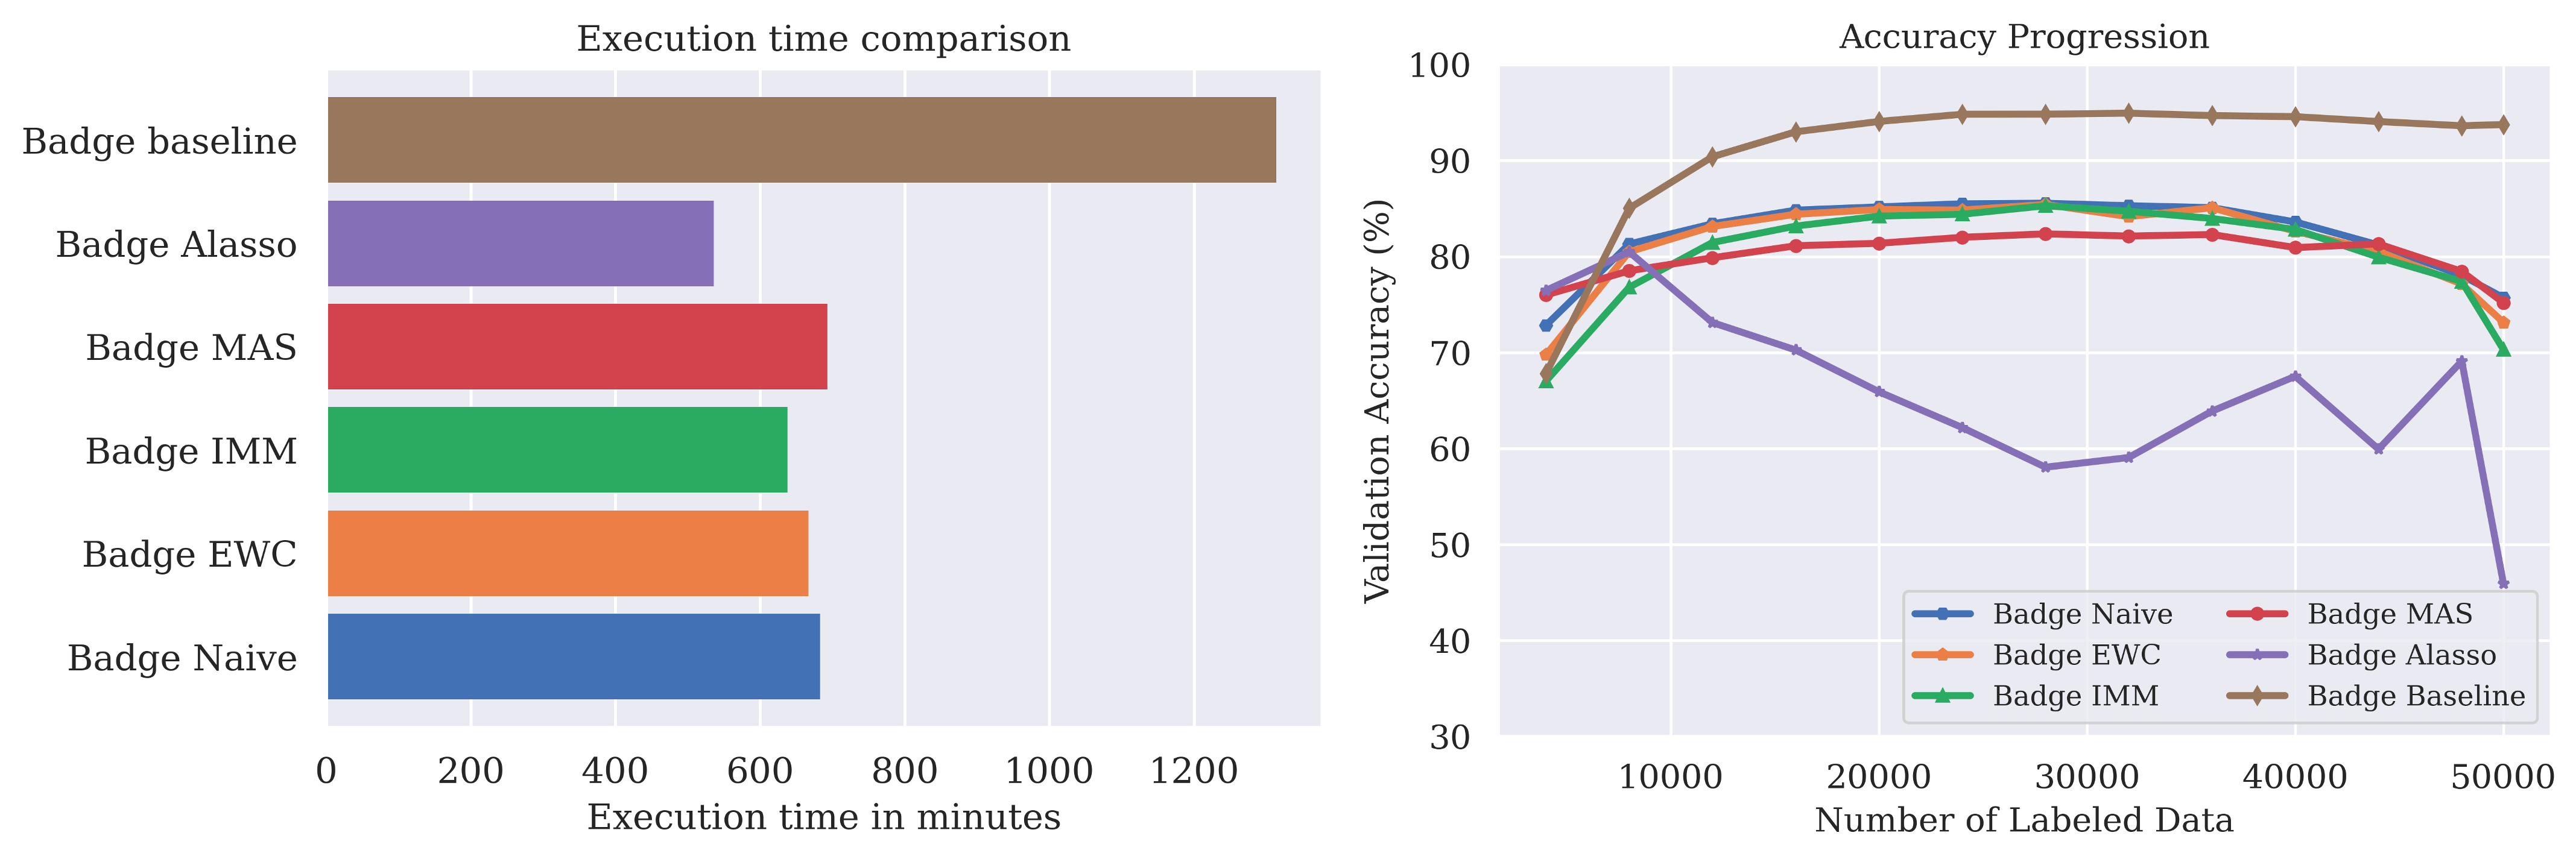
\includegraphics[width=\linewidth]{images/results_CAL/Badge_CAL_4000b.png}
    \caption[Continual Active Learning Badge 4000 batch size]{E}
    \label{fig:Evaluation:Results:CAL:Badge4000}
\end{figure}


\begin{figure} [ht]
    \centering
    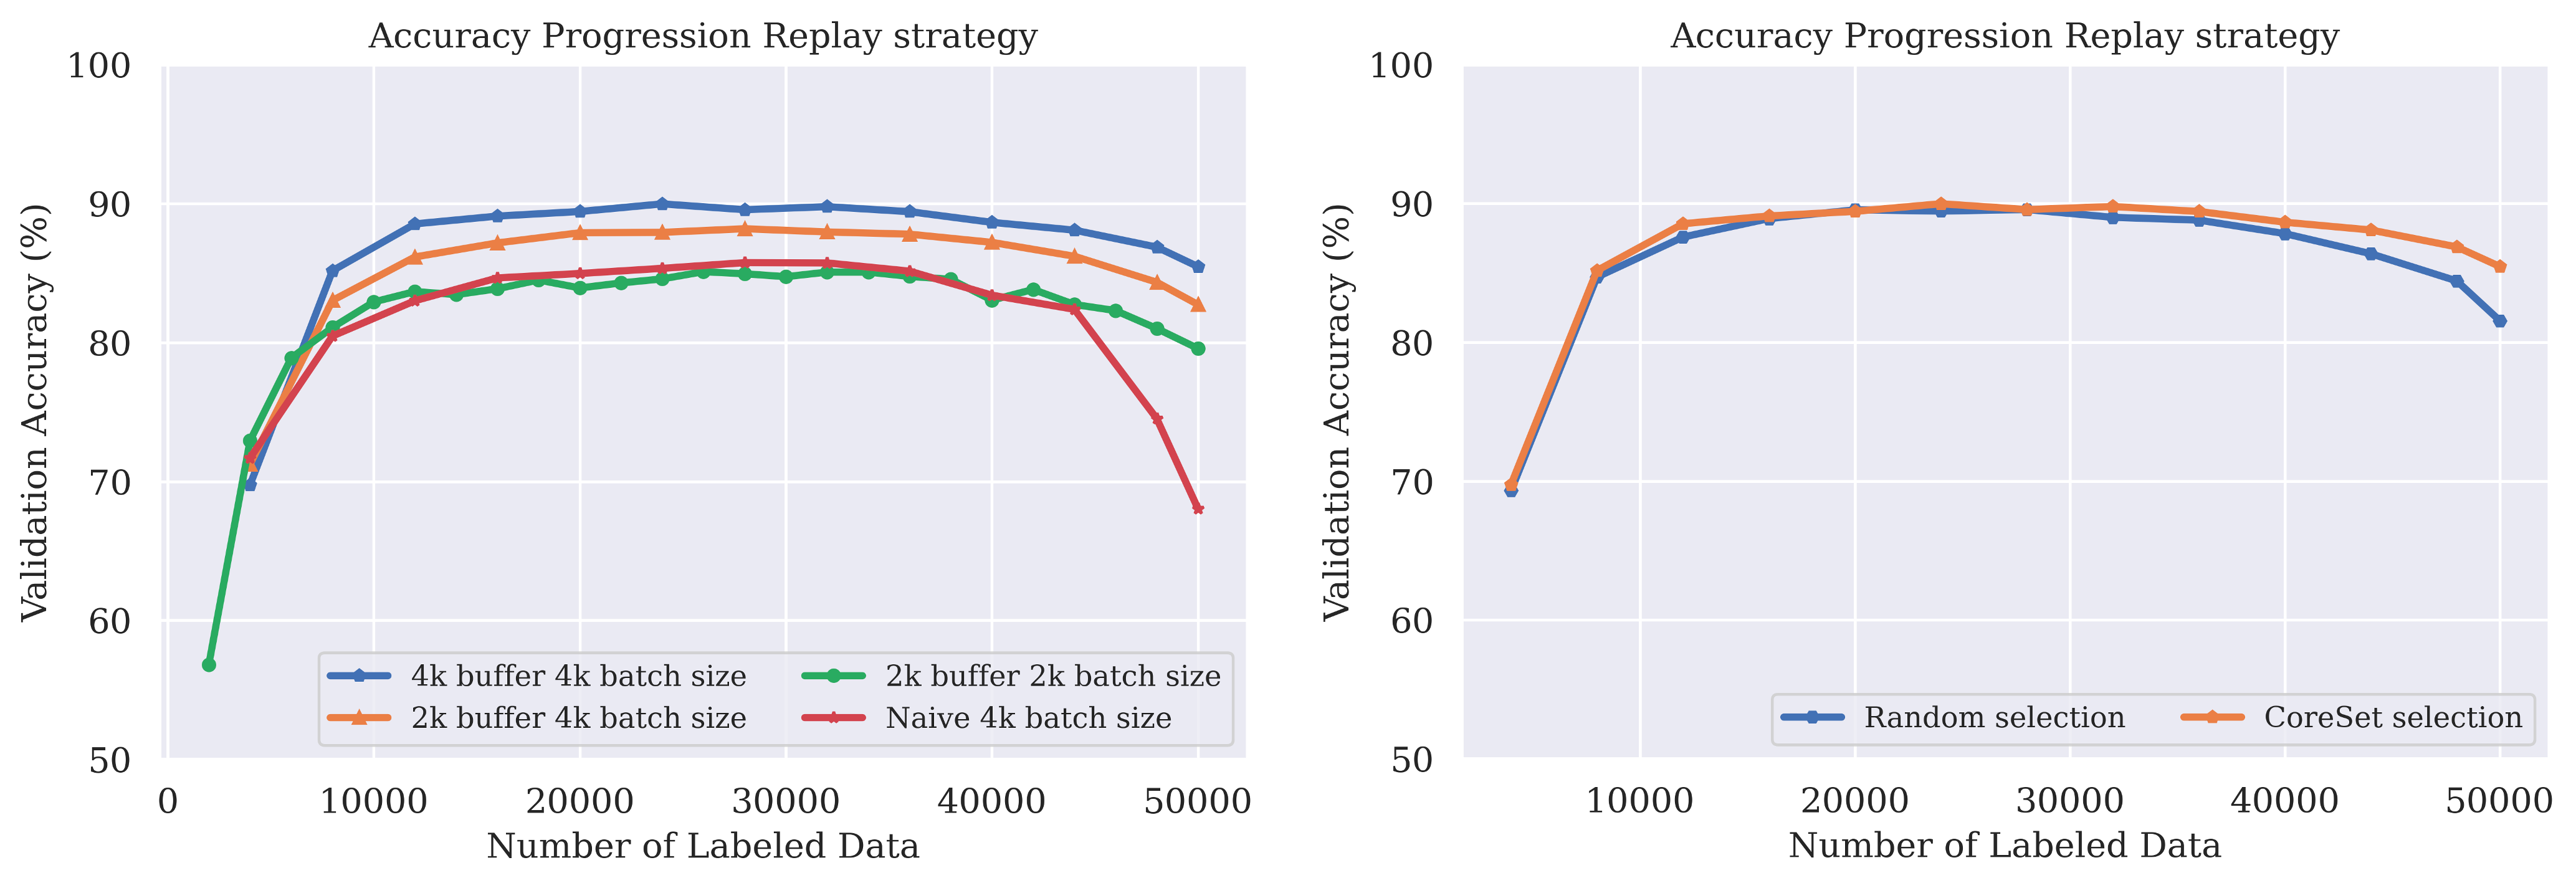
\includegraphics[width=\linewidth]{images/results_CAL/replay_CAL.png}
    \caption[Continual Active Learning Badge 4000 batch size]{E}
    \label{fig:Evaluation:Results:CAL:Replay}
\end{figure}

\begin{figure} [ht]
    \centering
    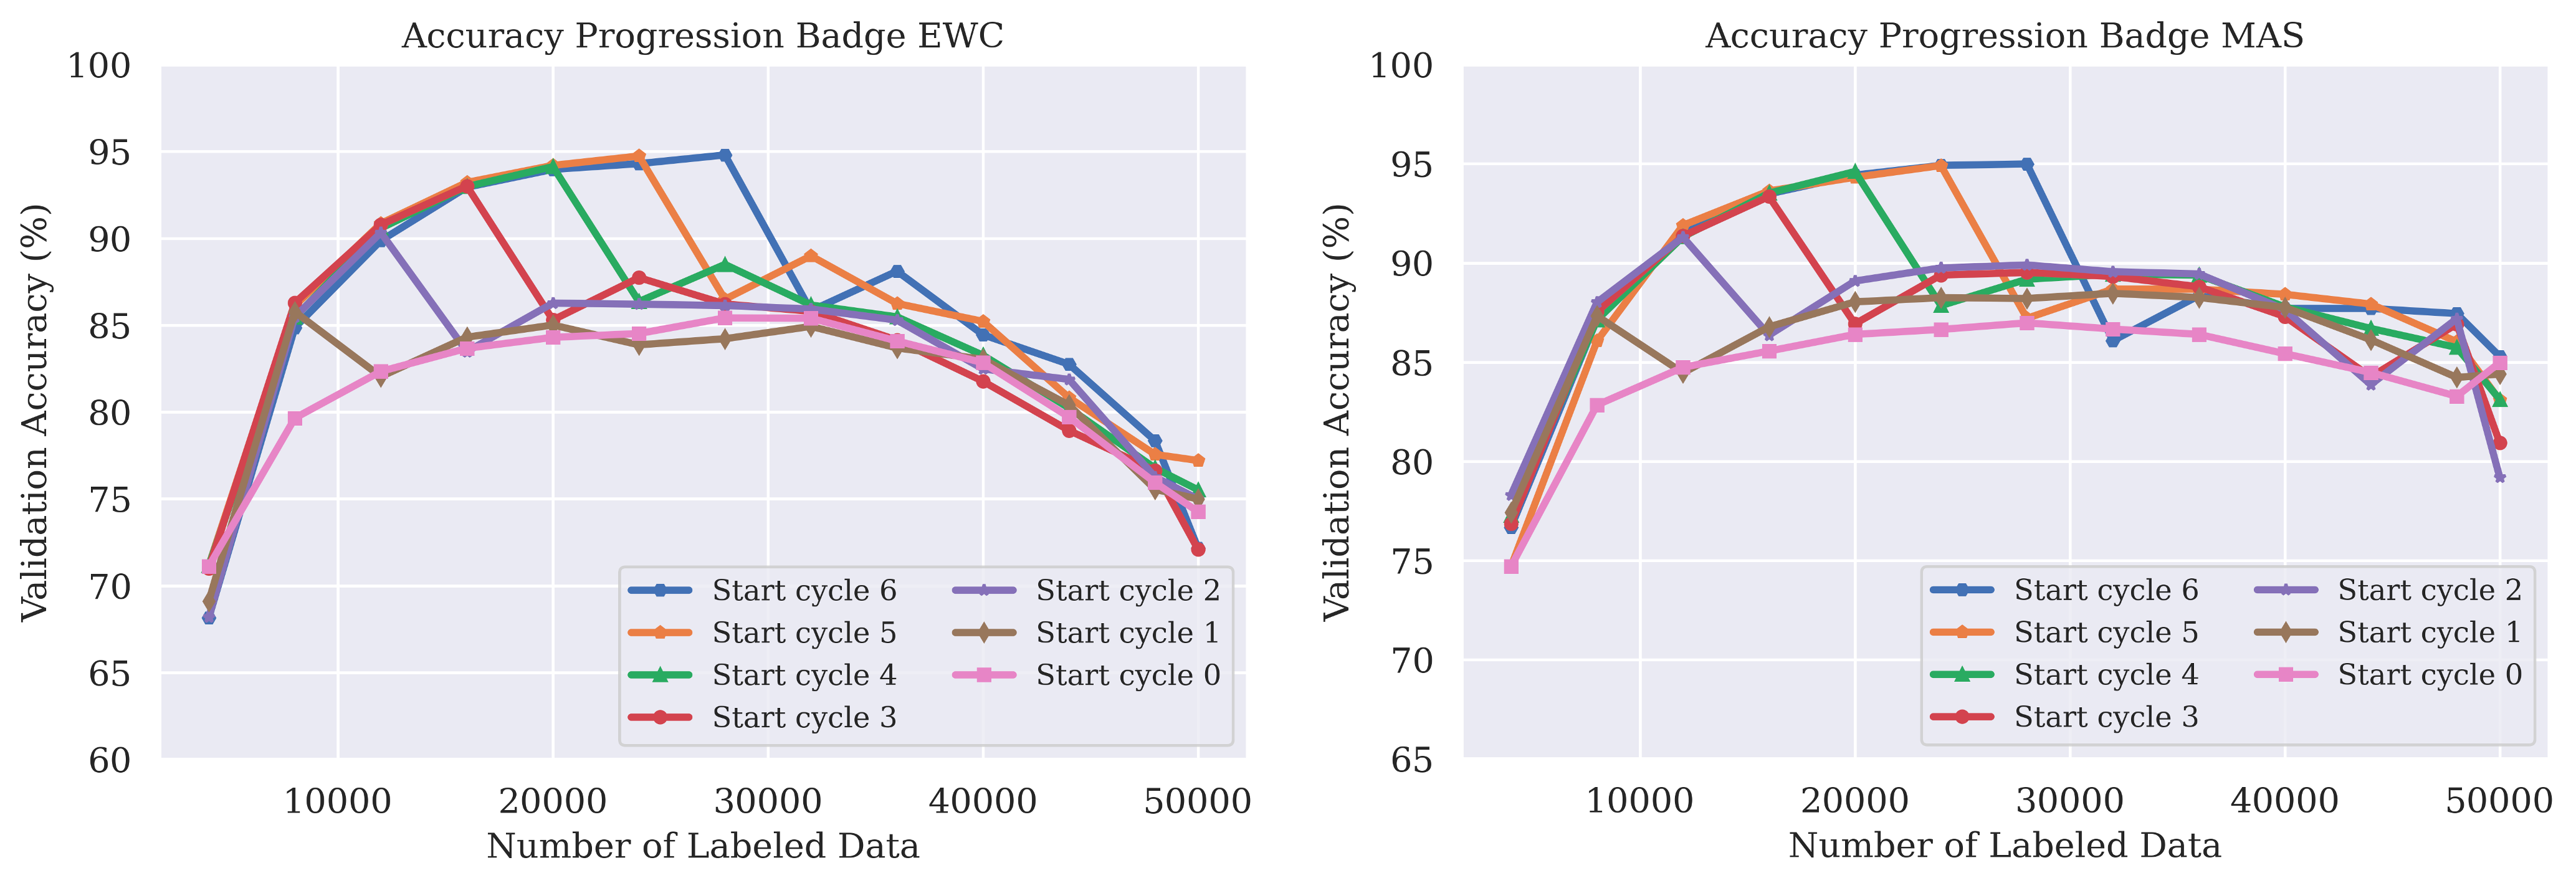
\includegraphics[width=\linewidth]{images/results_CAL/Delayed_start_CAL.png}
    \caption[Continual Active Learning Badge 4000 batch size]{E}
    \label{fig:Evaluation:Results:CAL:DelayedStart}
\end{figure}


\subsection{Results for Continual Active Learning for Model Stealing}
\label{sec:Evaluation:Results:CALMS}


\section{Discussion}
\label{sec:Evaluation:ThirdSection}
% Was war das Ziel? Was wurde (nicht) erreicht?

\dots
%% ---------------------
%% | / Example content |
%% ---------------------